% =====================================================================
%  Cadenza — Documento principal de tesis (versión fusionada)
%  Plantilla: IEEEtran (conference)
%
%  Versión 2 (2026-11-19): contrastada con el repositorio Cadenza
%  (rama dev, 593c6ca). Ver INFORME_CAMBIOS.md.
%
%  Contenido:
%    I.    Introducción                 VII.  Arquitectura de la solución
%    II.   Planteamiento del problema   VIII. Prototipo funcional (MVP)
%    III.  Justificación                IX.   Resultados
%    IV.   Objetivos                    X.    Instrumento de evaluación
%    V.    Metodología de la RSL        XI.   Conclusiones
%    VI.   Marco teórico
%
%  Convenciones de los comentarios:
%    % fuente: ...     de dónde sale cada cifra o afirmación (archivo del
%                      repositorio, ADR o issue de sebdavid3/Cadenza).
%    % PENDIENTE: ...  lo que falta verificar o decidir antes de entregar.
%
%  Bibliografía: UNA SOLA lista al final, numerada en orden de primera cita
%  (estilo IEEE); todas las citas del texto apuntan a esas claves.
%
%  Compilación (pdflatex, sin bibtex — bibliografía inline):
%    pdflatex main   (dos pasadas, para resolver \cite y \ref)
% =====================================================================
\documentclass[conference]{IEEEtran}
\IEEEoverridecommandlockouts

\usepackage{cite}
\usepackage{amsmath,amssymb,amsfonts}
\usepackage{graphicx}
\usepackage{textcomp}
\usepackage{xcolor}
\usepackage{array}
\usepackage{url} % faltaba: el texto usa \url
% Paquetes para español:
\usepackage[utf8]{inputenc}
\usepackage[T1]{fontenc}
\usepackage[spanish,es-tabla]{babel}
% Diagramas (árbol del problema):
\usepackage{tikz}
\usetikzlibrary{positioning,arrows.meta,fit,backgrounds}
% Paleta común de las figuras: morados del sistema visual de Cadenza
% (apps/web/src/styles/tokens.css: acento #7A2CF0, tinta atenuada #4A4950).
\definecolor{cadA}{HTML}{2A1263} % reconocimiento: violeta noche
\definecolor{cadB}{HTML}{5320B8} % validación: violeta profundo
\definecolor{cadC}{HTML}{7A2CF0} % corrección: el acento de Cadenza
\definecolor{cadD}{HTML}{A6379F} % aprendizaje: púrpura magenta
\definecolor{cadG}{HTML}{4A4950} % neutro: tinta atenuada

\begin{document}

% ---------------------------------------------------------------------
% TÍTULO
% ---------------------------------------------------------------------
\title{Cadenza: reconocimiento, validación y aprendizaje en la
digitalización de partituras}

% ---------------------------------------------------------------------
% AUTORES
% ---------------------------------------------------------------------
\author{\IEEEauthorblockN{Andrés Carrero Martínez}
\IEEEauthorblockA{\textit{Ingeniería de Sistemas} \\
\textit{Universidad del Norte}\\
Barranquilla, Colombia \\
aacarrero@uninorte.edu.co}
\and
\IEEEauthorblockN{Sebastián Ibáñez Ríos}
\IEEEauthorblockA{\textit{Ingeniería de Sistemas} \\
\textit{Universidad del Norte}\\
Barranquilla, Colombia \\
sdibanez@uninorte.edu.co}
\and
\IEEEauthorblockN{Carlos Herrera Rojano}
\IEEEauthorblockA{\textit{Ingeniería de Sistemas} \\
\textit{Universidad del Norte}\\
Barranquilla, Colombia \\
carlosrojano@uninorte.edu.co}
}

\maketitle
% ---------------------------------------------------------------------
% FIGURA 1: árbol del problema (flotante a página completa).
% Se declara aquí arriba para que LaTeX la ubique al inicio de las
% primeras páginas y NO caiga sobre la bibliografía al final.
% ---------------------------------------------------------------------
\begin{figure*}[!t]
    \centering
    \begin{tikzpicture}[
        % Configuración general de fuente y distancias
        font=\sffamily\scriptsize,
        node distance=0.4cm and 1.5cm,
        % Estilo base para todas las cajas
        caja/.style={draw, thick, align=center, inner sep=6pt, rounded corners=3pt},
        % Estilos específicos
        cat/.style={caja, fill=cadA, draw=cadA, text=white, font=\scriptsize\bfseries, text width=5cm},
        subcausa/.style={caja, fill=cadA!7, draw=cadA, text width=5cm, align=left, font=\tiny},
        problema/.style={caja, fill=cadD!10, draw=cadD, very thick, text width=5cm, font=\scriptsize, inner sep=8pt},
        efecto/.style={caja, fill=cadC!7, draw=cadC, text width=4.8cm},
        % Estilo de las flechas
        flecha/.style={-{Stealth[scale=1.2]}, thick, draw=cadG}
    ]

    % ===============================
    % CAUSAS (Columna Izquierda)
    % ===============================
    
    % Causa 1
    \node[cat] (cat1) {1. Modelos de Reconocimiento OMR};
    \node[subcausa, below=0.1cm of cat1] (c1) {$\bullet$ \emph{Domain shift} en CRNNs/Transformers sobre páginas completas.\\ $\bullet$ Degradación del reconocimiento en manuscritos modernos por la variabilidad del trazo.};

    % Causa 2
    \node[cat, below=0.4cm of c1] (cat2) {2. Validación Semántica Simbólica};
    \node[subcausa, below=0.1cm of cat2] (c2) {$\bullet$ Inferencia probabilística sin garantías sintácticas.\\ $\bullet$ Ausencia de parsers de teoría musical (reglas \emph{music21}).};

    % Causa 3
    \node[cat, below=0.4cm of c2] (cat3) {3. Ciclo de Aprendizaje Activo};
    \node[subcausa, below=0.1cm of cat3] (c3) {$\bullet$ Descarte de retroalimentación \emph{Human-in-the-Loop} (HITL).\\ $\bullet$ Falta de pipelines de reentrenamiento a partir de las correcciones del usuario.};

    % ===============================
    % PROBLEMA CENTRAL (Columna Central)
    % ===============================
    
    % Se posiciona a la derecha de Causa 2 para quedar centrado verticalmente
    \node[problema, right=1.2cm of c2] (p) {\textbf{Ineficiencia y fragmentación tecnológica en OMR:}\\[6pt] Elevado esfuerzo de corrección manual debido a la desconexión entre modelos neuronales, validadores formales y reentrenamiento activo};

    % ===============================
    % EFECTOS (Columna Derecha)
    % ===============================
    
    % Se posiciona el efecto central y luego los demás arriba y abajo
    \node[efecto, right=1.2cm of p] (e2) {\textbf{Corrupción de esquemas MusicXML:}\\ Archivos no reproducibles con compases rítmicamente desbalanceados};
    \node[efecto, above=0.5cm of e2] (e1) {\textbf{Bajo rendimiento en Benchmarks:}\\ Altas tasas de error SER y OMR-NED en corpus estándar (PrIMuS, SMB, MUSCIMA++)};
    \node[efecto, below=0.5cm of e2] (e3) {\textbf{Desperdicio de supervisión:}\\ Pérdida de pares de corrección de alto costo para el aprendizaje continuo};

    % ===============================
    % CONEXIONES (Flechas)
    % ===============================
    
    % Conexiones de Causas a Problema (curvas de salida 0 grados, entrada 180 grados)
    \draw[flecha] (c1.east) to[out=0, in=180] (p.west);
    \draw[flecha] (c2.east) to[out=0, in=180] (p.west);
    \draw[flecha] (c3.east) to[out=0, in=180] (p.west);

    % Conexiones de Problema a Efectos
    \draw[flecha] (p.east) to[out=0, in=180] (e1.west);
    \draw[flecha] (p.east) to[out=0, in=180] (e2.west);
    \draw[flecha] (p.east) to[out=0, in=180] (e3.west);

    \end{tikzpicture}
    \caption{Árbol de problemas tecnológico y multidimensional: modelos de reconocimiento, validación simbólica y ciclo de aprendizaje activo.}
    \label{fig:arbol}
\end{figure*}

% =====================================================================
% I. INTRODUCCIÓN
% =====================================================================
\section{Introducción}

La digitalización del patrimonio musical constituye una necesidad
creciente para archivos, bibliotecas, academias y agrupaciones musicales
que conservan partituras físicas en papel. El reconocimiento óptico de
música (OMR, por sus siglas en inglés) es la disciplina que aborda la
conversión automática de imágenes de partituras en representaciones
simbólicas editables, y ha sido objeto de investigación durante más de
cinco décadas \cite{omr2020}, evolucionando desde sistemas basados en
reglas hasta \emph{pipelines} de aprendizaje profundo que transcriben
partituras completas de forma automática
\cite{rebelo2012,calvo2018,riosvila2026}.

A pesar de estos avances, los sistemas OMR modernos cometen errores que
impiden su uso directo en entornos reales: notas con alturas o duraciones
incorrectas, compases desbalanceados, armaduras inconsistentes y símbolos
omitidos \cite{calvo2018}. Los modelos de reconocimiento se estudian
predominantemente desde la precisión de su salida automática, mientras
que la integración del reconocimiento en el trabajo práctico de un
transcriptor ha recibido mucha menos atención \cite{rizo2023}. Como
consecuencia, quien digitaliza partituras termina revisando manualmente
cada símbolo en un editor musical convencional, un proceso tan lento como
la transcripción manual, o acepta resultados erróneos sin verificarlos.
En el caso de los manuscritos musicales modernos, esta situación se
agudiza, pues la variabilidad de la escritura degrada aún más la
confiabilidad del reconocimiento automático \cite{ricordi2024}. Del mismo
modo, el aprovechamiento de las correcciones del usuario para mejorar el
sistema mediante ciclos de aprendizaje activo sigue siendo poco explorado
en OMR, donde los primeros estudios arrojan resultados incluso
contradictorios \cite{mlsp2025}.

En el contexto internacional, archivos y bibliotecas conservan colecciones
de partituras impresas y escritas a mano que requieren digitalización para
su preservación, consulta y difusión. La transcripción manual de estas
colecciones representa un costo de tiempo considerable, y las herramientas
de reconocimiento existentes no ofrecen un flujo de trabajo que garantice
la calidad del resultado. La digitalización de colecciones musicales ha
sido abordada recientemente desde la archivística con metodologías de
anotación y clasificación automática \cite{ricordi2024}; aun así,
faltan herramientas de transcripción asistida pensadas para el trabajo
del transcriptor.

La comunidad de OMR dispone de conjuntos de datos públicos de referencia.
PrIMuS y Camera-PrIMuS \cite{calvo2018,cameraprimus2018} proveen 87\,678
\emph{incipits} de partituras impresas monofónicas, el segundo con
distorsiones que simulan fotografías tomadas en condiciones reales, y
\emph{ground truth} simbólico en múltiples formatos. El Sheet Music
Benchmark (SMB) \cite{smb2025} estandariza la evaluación con 685 páginas
que incluyen monofonía y \emph{pianoform}, divisiones predefinidas y una
métrica de error detallada por elemento musical (OMR-NED). Para la notación
manuscrita, MUSCIMA++ \cite{muscima2017} ofrece más de 91\,000 símbolos
anotados sobre partituras escritas a mano por músicos actuales. La
disponibilidad de \emph{ground truth} en estos conjuntos permite evaluar un
sistema de forma cuantitativa y reproducible. En este trabajo, la
evaluación se realizó sobre PrIMuS y Camera-PrIMuS y sobre un conjunto de
doce páginas impresas de voz con piano; SMB y MUSCIMA++, previstos en el
planteamiento, no llegaron a evaluarse.
% fuente: issue #102 (decisión del 2026-11-19); results/ (exp_03, exp_12, exp_15, exp_18)

Desde el punto de vista disciplinar, un sistema de digitalización
asistida de partituras puede estructurarse sobre tres pilares: el
\emph{pipeline} clásico de OMR (preprocesado, detección de pentagramas,
detección y clasificación de símbolos, ensamblaje y reconstrucción
musical \cite{omr2020}), la validación de la salida
mediante reglas de teoría musical \cite{cuthbert2010}, y la corrección
asistida por un humano en el ciclo \cite{amershi2014}. La validación
automática permite detectar errores estructurales (métrica, duraciones,
armaduras) sin intervención humana, reduciendo el espacio de revisión a
los puntos sospechosos. El aprendizaje activo complementa el ciclo al
seleccionar qué correcciones del usuario tienen mayor valor para mejorar
el reconocimiento \cite{settles2009}.

En este contexto, el presente proyecto propone el diseño e
implementación de \textbf{Cadenza}, una plataforma de digitalización
asistida de partituras que integra cuatro componentes: un modelo OMR base
(HOMR \cite{homr2024}) encargado de la transcripción automática a
MusicXML; un motor de validación basado en reglas musicales que detecta y
señala errores probables; una interfaz de corrección asistida que permite
al usuario revisar y corregir la transcripción junto a la imagen original,
con reproducción de la partitura digitalizada; y un mecanismo de
aprendizaje que aprovecha las correcciones del usuario. El planteamiento
inicial preveía un ciclo de aprendizaje activo que reentrenara el
reconocedor y un alcance que incluía partituras impresas y manuscritas
actuales, monofónicas o de piano simple. El sistema entregado concreta ese
mecanismo como una capa de sugerencias que aprende de las correcciones sin
reentrenar el modelo, y su alcance probado se limita a partituras
impresas: una línea, piano y voz con piano. Las orquestaciones completas y
los manuscritos históricos quedaron excluidos desde el inicio.
% fuente: docs/adr/ADR-0036:26-32; issue #103; docs/investigaciones/INV-0002; docs/phases/plan_de_cierre/README.md:23-63

Este es un proyecto de ingeniería: su aporte es el sistema construido y la
forma en que se verificó. El resto del documento se organiza así: tras el
planteamiento del problema, la justificación y los objetivos, se presentan
la revisión de literatura y el marco teórico que fundamentan el diseño;
siguen la arquitectura de la solución y el prototipo funcional; después,
los resultados de la verificación y la evaluación de calidad del
prototipo; y cierran las conclusiones.

% =====================================================================
% II. PLANTEAMIENTO DEL PROBLEMA
% =====================================================================

\section{Planteamiento del Problema}

En la práctica, la digitalización de partituras continúa siendo un
proceso predominantemente reactivo y dependiente del esfuerzo humano.
Aunque el reconocimiento óptico de música ha evolucionado desde sistemas
basados en reglas hasta \emph{pipelines} de aprendizaje profundo capaces de
transcribir páginas completas de forma automática
\cite{omr2020,calvo2018,riosvila2026}, su salida aún comete
errores frecuentes que impiden usarla directamente \cite{calvo2018}: alturas
o duraciones incorrectas, compases desbalanceados, armaduras inconsistentes
y símbolos omitidos. Por eso, quien digitaliza termina corrigiendo
símbolo por símbolo en un editor convencional, con un costo de tiempo
cercano al de la transcripción manual, o bien acepta resultados sin
verificación alguna. En el caso de los manuscritos modernos esta situación se
agrava: la irregularidad del trazo, la inclinación de las plicas y la
variabilidad geométrica de los símbolos degradan aún más la
confiabilidad del reconocimiento automático \cite{ricordi2024}.

Esta condición evidencia una brecha disciplinar: los modelos de
reconocimiento se estudian predominantemente desde la precisión de su
salida automática, mientras que su integración en el trabajo práctico
de un transcriptor ha recibido mucha menos atención \cite{rizo2023}. El
objeto de estudio de este proyecto es, por tanto, el diseño de un sistema
de información que resuelva la fragmentación actual entre tres
dimensiones que hoy operan de manera aislada: (i) los \emph{modelos de
reconocimiento OMR}, evaluados casi exclusivamente mediante métricas de
precisión simbólica; (ii) las técnicas de \emph{validación musical},
capaces de detectar errores estructurales de métrica, duraciones y
armaduras mediante reglas de teoría musical sin intervención humana
\cite{cuthbert2010}; y (iii) los \emph{mecanismos de interacción humana},
que permiten al usuario corregir la transcripción sobre la imagen
original, pero cuyas correcciones, en los sistemas actuales, se descartan
sin alimentar con ellas la mejora progresiva del sistema mediante
aprendizaje activo, enfoque prácticamente inexplorado en OMR y con
resultados iniciales incluso contradictorios
\cite{amershi2014,settles2009,mlsp2025}.

A nivel de ingeniería, el problema se concreta en la inexistencia de una
plataforma tecnológica integrada que articule estas dimensiones, tal como
resume el árbol de problemas de la Figura~\ref{fig:arbol}. La
solución debe cumplir cinco requisitos de sistema: (i) transcribir la
imagen de una partitura a una representación simbólica editable y
conservar lo que leyó el motor; (ii) señalar los posibles errores de la
transcripción con reglas explicables, sin intervención humana; (iii)
permitir corregir sobre la partitura, junto a la imagen original, sin
perder ninguna edición; (iv) registrar cada corrección de forma trazable y
con permiso de uso, para aprovecharla después; y (v) operar como un
servicio web desplegable, seguro y mantenible. El cumplimiento de estos
requisitos se verifica con tres tipos de evidencia: pruebas automáticas
del software; mediciones reproducibles de la fidelidad de la
transcripción, con la tasa de error simbólico (\emph{Symbol Error Rate},
SER) y la distancia OMR-NED, y del desempeño de las reglas; y una
evaluación de calidad del producto con el modelo ISO/IEC~25010.

En el contexto regional, esta necesidad afecta a archivos, academias y
agrupaciones musicales que conservan colecciones de partituras impresas y
escritas a mano cuya transcripción manual representa costos de tiempo
considerables, y que cuentan únicamente con editores convencionales, sin
mecanismos de verificación automática ni de mejora continua. La
experiencia reciente de digitalización de colecciones musicales,
abordada con metodologías de anotación y clasificación automática
\cite{ricordi2024}, confirma que el problema es real y abordable desde la
ingeniería. A ello se suma que los conjuntos de datos públicos con
\emph{ground truth}, como PrIMuS/Camera-PrIMuS
\cite{calvo2018,cameraprimus2018}, Sheet
Music Benchmark \cite{smb2025} y MUSCIMA++ \cite{muscima2017}, permiten
evaluar la solución propuesta de forma cuantitativa y reproducible,
siguiendo los protocolos de la literatura de OMR.

\textbf{Pregunta de diseño:} \textquestiondown Cómo diseñar e implementar
una plataforma de digitalización asistida de partituras que integre
reconocimiento óptico de música, validación automática mediante reglas de
teoría musical, corrección interactiva y aprendizaje a partir de las
correcciones del usuario, de modo que su calidad pueda verificarse con
pruebas automáticas, con mediciones reproducibles de fidelidad y con un
modelo de calidad del software?
% Reformulada el 2026-11-19 por indicación del responsable, para un proyecto
% de grado de ingeniería.
% Redacción original (pregunta de investigación): «¿De qué manera el diseño e
% implementación de una plataforma de digitalización asistida de partituras,
% que integre reconocimiento óptico de música, validación automática mediante
% reglas de teoría musical y un ciclo de aprendizaje activo a partir de las
% correcciones del usuario, permite reducir el esfuerzo de revisión humana y
% mejorar la fidelidad de la transcripción digital (MusicXML/MIDI), medida en
% tasa de error simbólico y tiempo de edición, en partituras impresas y
% manuscritos modernos de complejidad monofónica o piano simple?». También
% se sustituyeron las variables independiente, mediadora y dependientes por
% los requisitos de sistema del párrafo anterior.

% =====================================================================
% III. Justificación 
% =====================================================================
\section{Justificación}
La digitalización de una partitura impresa sigue exigiendo trabajo manual.
Los sistemas de reconocimiento óptico de música han avanzado, pero su
salida todavía contiene errores de altura, de duración y de estructura que
impiden usarla sin revisión \cite{rebelo2012,calvo2018}. Quien necesita una
versión editable de una partitura debe elegir entre transcribirla a mano o
corregir, símbolo por símbolo, lo que produjo el reconocedor. Una
plataforma que integre el reconocimiento con la revisión se justifica
porque cambia ese trabajo: en lugar de recorrer toda la partitura, la
persona atiende los puntos que el sistema señala como sospechosos, junto a
la imagen original, y puede comprobar el resultado de oído.

La solución se justifica también por cómo aprovecha lo que ya existe. Las
reglas de teoría musical permiten detectar errores estructurales de forma
explicable, sin entrenar ningún modelo \cite{cuthbert2010}; y las
correcciones de la persona, que los flujos habituales descartan, son
información valiosa sobre los fallos del reconocedor \cite{amershi2014}.
Este proyecto las conserva de forma trazable y con permiso de uso, aprende
de ellas para proponer arreglos y las deja preparadas para mejorar el
reconocimiento más adelante. El beneficio alcanza a quienes migran
partituras impresas a formatos digitales, como músicos, docentes,
academias y agrupaciones, y a la enseñanza de la escritura musical. El
proyecto se limita a la notación impresa; la notación manuscrita, cuya
variabilidad degrada aún más el reconocimiento \cite{ricordi2024}, queda
como extensión natural.

% =====================================================================
% IV. Objetivos
% =====================================================================

\section{Objetivos}

\subsection{Objetivo general}
\label{sec:objetivo-general}

Diseñar e implementar una plataforma de digitalización asistida de partituras que integre reconocimiento óptico de música, validación automática mediante reglas de teoría musical, corrección interactiva y aprendizaje activo.

\subsection{Objetivos específicos}
\label{sec:objetivos-especificos}

\begin{enumerate}
    \item Analizar las técnicas de reconocimiento óptico de música, validación basada en reglas musicales y aprendizaje activo aplicables a la digitalización de partituras impresas y manuscritas modernas, con el propósito de establecer los fundamentos técnicos y metodológicos de la plataforma.

    \item Diseñar una arquitectura de software que integre un modelo OMR, un módulo de validación automática de errores musicales, una interfaz de corrección asistida y un mecanismo de aprendizaje activo basado en las correcciones realizadas por el usuario.

    \item Implementar un prototipo funcional de la plataforma Cadenza capaz de procesar imágenes de partituras, generar transcripciones en formatos simbólicos como MusicXML/MIDI, identificar inconsistencias mediante reglas musicales y permitir la corrección interactiva de los resultados.

    \item Desarrollar un mecanismo de aprendizaje activo que utilice las correcciones realizadas por los usuarios para seleccionar muestras relevantes y contribuir al mejoramiento progresivo del reconocimiento de partituras.

\end{enumerate}

% Nota: los objetivos no se han reescrito. Dos discrepancias conocidas (issue #270):
%  1) el diagrama original (diagrama_#.jpeg, ya sustituido) mostraba otros cuatro objetivos,
%     distintos de los de esta lista (desarrollar un sistema OMR con
%     metadatos de confianza y posición; motor de validación; interfaz de
%     corrección priorizada; mecanismo de aprendizaje activo que mejore
%     iterativamente el modelo OMR) y un «criterio de validación y éxito»
%     (mejora en OMR-NED o F1 en PrIMuS, SMB y MUSCIMA++; reducción del
%     tiempo frente a la transcripción manual; SUS >= 70; mejora del modelo
%     en iteraciones sucesivas) que no se midió.
%  2) El repositorio cita un «Objetivo Específico 5» (evaluación experimental
%     frente a una línea base; docs/experimentos/protocolo_medicion_esfuerzo.md:15-16)
%     que no aparece aquí.
La Figura~\ref{fig:alineacion-objetivos} resume la relación entre el problema
formulado, los objetivos, la arquitectura de la solución, el prototipo y la
evidencia reunida.

% Figura dibujada en TikZ (sustituye a diagrama_#.jpeg). Los objetivos son
% los del texto de esta sección, abreviados.
% Si cambian los objetivos, actualizar la segunda tarjeta.
\begin{figure*}[!t]
    \centering
    \begin{tikzpicture}[
        font=\sffamily\scriptsize,
        cuerpo/.style={draw=#1, line width=0.8pt, rounded corners=3pt, fill=#1!7, text width=3.2cm, align=left, inner sep=5pt, minimum height=27mm, anchor=north},
        cabeza/.style={fill=#1, text=white, font=\sffamily\scriptsize\bfseries, rounded corners=3pt, text width=3.2cm, align=center, inner sep=5pt, minimum height=8mm, anchor=south},
        num/.style={circle, fill=white, text=#1, font=\sffamily\scriptsize\bfseries, inner sep=1.6pt, minimum size=4.6mm},
        pildora/.style={draw=#1, line width=0.7pt, fill=white, rounded corners=6.5pt, inner xsep=6pt, inner ysep=3.5pt, align=center, text width=3.2cm},
        flujo/.style={-{Stealth[scale=1.25]}, line width=1.1pt, draw=cadG},
        rot/.style={font=\sffamily\tiny, align=center, text=cadG, inner sep=2pt}
    ]
    \node[cabeza=cadA] (h1) at (0,0) {\hspace{5mm}Problema};
    \node[cabeza=cadB] (h2) at (4.6,0) {\hspace{5mm}Objetivos};
    \node[cabeza=cadC] (h3) at (9.2,0) {\hspace{5mm}Arquitectura};
    \node[cabeza=cadD] (h4) at (13.8,0) {\hspace{5mm}Prototipo};
    \node[num=cadA] at ([xshift=5.2mm]h1.west) {1};
    \node[num=cadB] at ([xshift=5.2mm]h2.west) {2};
    \node[num=cadC] at ([xshift=5.2mm]h3.west) {3};
    \node[num=cadD] at ([xshift=5.2mm]h4.west) {4};

    \node[cuerpo=cadA] (b1) at (0,-0.12) {$\bullet$ La salida del OMR tiene errores\\ $\bullet$ Se revisa símbolo por símbolo\\ $\bullet$ Las correcciones no se aprovechan};
    \node[cuerpo=cadB] (b2) at (4.6,-0.12) {1. Analizar las técnicas\\ 2. Diseñar la arquitectura\\ 3. Implementar el prototipo\\ 4. Aprendizaje activo a partir de las correcciones};
    \node[cuerpo=cadC] (b3) at (9.2,-0.12) {$\bullet$ Motor OMR (HOMR)\\ $\bullet$ Reglas de validación\\ $\bullet$ Interfaz de corrección\\ $\bullet$ Registro de ediciones\\ $\bullet$ Capa de sugerencias};
    \node[cuerpo=cadD] (b4) at (13.8,-0.12) {$\bullet$ Subir y transcribir\\ $\bullet$ Señalar posibles errores\\ $\bullet$ Corregir sobre la partitura\\ $\bullet$ Escuchar y exportar};

    \draw[flujo] (b1.east) -- node[rot, above=1.5pt] {motiva} (b2.west);
    \draw[flujo] (b2.east) -- node[rot, above=1.5pt] {definen} (b3.west);
    \draw[flujo] (b3.east) -- node[rot, above=1.5pt] {se realiza\\en} (b4.west);

    % evidencia
    \node[pildora=cadA] (e1) at (0,-4.55) {SER y OMR-NED en PrIMuS y Camera-PrIMuS};
    \node[pildora=cadB] (e2) at (4.6,-4.55) {Precisión y sensibilidad de las reglas};
    \node[pildora=cadC] (e3) at (9.2,-4.55) {Calidad del software: ISO/IEC 25010};
    \node[pildora=cadD] (e4) at (13.8,-4.55) {Acierto de la primera sugerencia};
    \node[font=\sffamily\scriptsize\bfseries, text=cadG, anchor=south west] (te) at ([yshift=1.5mm]e1.north west) {Evidencia reunida};
    \begin{scope}[on background layer]
        \node[draw=cadG, line width=0.7pt, rounded corners=3pt, fill=cadG!6, inner sep=5pt, fit=(te)(e1)(e4)] (me) {};
    \end{scope}
    \draw[flujo] (b3.south) -- (b3.south |- me.north);
    \draw[flujo] (b4.south) -- (b4.south |- me.north);
    \end{tikzpicture}
    \caption{Alineación entre el problema, los objetivos, la arquitectura y el prototipo, con la evidencia reunida sobre la solución.}
    \label{fig:alineacion-objetivos}
\end{figure*}
% =====================================================================
% V. METODOLOGÍA DE REVISIÓN SISTEMÁTICA (RSL)
% =====================================================================
\section{Metodología de Revisión Sistemática (RSL)}
\label{sec:metodologia-rsl}

Para la construcción del marco teórico y la fundamentación conceptual y técnica de la plataforma Cadenza, se realizó una Revisión Sistemática de Literatura (RSL) siguiendo las directrices metodológicas del protocolo PRISMA 2020 \cite{prisma2020}.

\subsection{Estrategia de Búsqueda}
\label{sec:estrategia-busqueda}

Se realizaron búsquedas exhaustivas en las principales bases de datos académicas y repositorios científicos de alta indexación en las áreas de ciencias de la computación, procesamiento de señales e informática musical: IEEE Xplore Digital Library, Scopus (Elsevier), ACM Digital Library, SpringerLink, ScienceDirect, Google Scholar y las actas de conferencias de la International Society for Music Information Retrieval (ISMIR).

El período de búsqueda comprendió la producción científica entre enero de 2016 y el año en curso (2026), capturando una década de avances tecnológicos. Se estructuró una cadena de búsqueda booleana orientada a identificar trabajos que combinaran modelos neuronales, validación y flujos interactivos:

% \textquotedbl en lugar de " : babel-spanish trata " como atajo activo y
% deformaba la cadena en el PDF.
\begin{quote}
\footnotesize\raggedright
\texttt{(\textquotedbl optical music recognition\textquotedbl{} OR \textquotedbl OMR\textquotedbl) AND (\textquotedbl deep learning\textquotedbl{} OR \textquotedbl neural network\textquotedbl{} OR \textquotedbl interactive\textquotedbl{} OR \textquotedbl validation\textquotedbl{} OR \textquotedbl human-in-the-loop\textquotedbl{} OR \textquotedbl active learning\textquotedbl)}
\end{quote}

\subsection{Criterios de Selección}
\label{sec:criterios-seleccion}

Se aplicaron filtros estrictos para garantizar la calidad, actualidad y pertinencia de las fuentes respecto a los objetivos de Cadenza, como se detalla en la Tabla~\ref{tab:criterios-prisma}.

\begin{table}[htbp]
\caption{Criterios de Inclusión y Exclusión}
\label{tab:criterios-prisma}
\centering
\footnotesize
\begin{tabular}{|p{3.8cm}|p{3.8cm}|}
\hline
\textbf{Criterios de Inclusión} & \textbf{Criterios de Exclusión} \\
\hline
Artículos publicados entre 2016 y 2026 en revistas indexadas o conferencias internacionales con revisión por pares. & Artículos de opinión, cartas al editor, reportes preliminares o resúmenes sin texto completo accesible. \\
\hline
Estudios enfocados en reconocimiento óptico de música (OMR) mediante técnicas de \emph{Deep Learning} (CNN, CRNN, Transformers, SSM/Mamba-2). & Tecnologías obsoletas, pipelines segmentados tradicionales o sistemas basados exclusivamente en audio (AMT). \\
\hline
Propuestas sobre interfaces \emph{Human-in-the-Loop} (HITL), edición interactiva asistida o aprendizaje activo en documentos. & Estudios sobre manuscritos históricos medievales o notaciones antiguas (mensural/canto llano). \\
\hline
Mecanismos de validación sintáctica, consistencia de reglas musicales y posprocesamiento simbólico. & Software comercial propietario o patentes sin metodología reproducible ni código/datos abiertos. \\
\hline
Investigaciones que introduzcan o utilicen datasets públicos con \emph{ground truth} y métricas cuantitativas (SER, OMR-NED). & Documentos que no aporten a la digitalización de partituras en notación moderna. \\
\hline
Fuentes en idioma inglés y español. & Registros duplicados o reportes metodológicamente deficientes. \\
\hline
\end{tabular}
\end{table}

\subsection{Resultados del Flujo PRISMA}
\label{sec:resultados-prisma}

El proceso de selección de la información siguió el diagrama de flujo PRISMA 2020 \cite{prisma2020}, organizado aquí en cuatro etapas (identificación, cribado, evaluación de elegibilidad e inclusión), resultando en la selección final de 31 estudios primarios a partir de 458 registros inicialmente identificados. La Tabla~\ref{tab:resumen-prisma} resume cuantitativamente los resultados obtenidos en cada etapa con el correspondiente detalle de exclusión.

\begin{table}[htbp]
\caption{Tabla Resumen del Flujo PRISMA}
\label{tab:resumen-prisma}
\centering
\footnotesize
\begin{tabular}{|l|p{4.8cm}|c|}
\hline
\textbf{Fase PRISMA} & \textbf{Detalle del Proceso} & \textbf{Cant.} \\
\hline
\textbf{Identificación} & Registros identificados en bases de datos (Scopus: 72, IEEE Xplore: 55, SpringerLink: 65, ACM DL: 48, ScienceDirect: 40, Google Scholar: 140, ISMIR: 38) & 458 \\
\cline{2-3}
& \emph{(-) Registros duplicados eliminados} & 158 \\
\hline
\textbf{Cribado} & Registros cribados por título y resumen & 300 \\
\cline{2-3}
& \emph{(-) Excluidos por no ser relevantes} & 230 \\
\hline
\textbf{Elegibilidad} & Artículos de texto completo evaluados & 70 \\
\cline{2-3}
& \emph{(-) Excluidos a texto completo:} & 39 \\
& \quad $\bullet$ Sin dataset ni código público accesible (18) & \\
& \quad $\bullet$ Notación no occidental o histórica (11) & \\
& \quad $\bullet$ Pipelines segmentados clásicos obsoletos (10) & \\
\hline
\textbf{Inclusión} & \textbf{Estudios incluidos en la síntesis} & \textbf{31} \\
\hline
\end{tabular}
\end{table}

\subsection{Síntesis Temática y Clasificación de la Literatura}
\label{sec:sintesis-literatura}

% fuente de las cifras PRISMA: docs/revision-literatura-prisma.md:76-118 (458, 158, 300, 230, 70, 39, 31)
Los 31 estudios primarios seleccionados fueron organizados y sintetizados a lo largo de siete ejes temáticos fundamentales, los cuales articulan directamente cada módulo arquitectural de Cadenza. Las especificaciones de formatos y las herramientas de software citadas (MusicXML, MIDI, oemer, HOMR) se emplean como fuentes de apoyo y no se contabilizan entre los estudios primarios.

\subsubsection{OMR y Estado del Arte}
Los \emph{surveys} fundamentales de Calvo-Zaragoza et al. \cite{omr2020} y Rebelo et al. \cite{rebelo2012} establecen la taxonomía clásica del OMR en cuatro etapas: preprocesamiento, detección de pentagramas y glifos, clasificación y ensamblaje sintáctico. Estos antecedentes evidencian la transición de los enfoques heurísticos segmentados hacia sistemas de código abierto basados en aprendizaje profundo como oemer \cite{oemer2021} y HOMR \cite{homr2024}, identificando como reto persistente la corrección de errores estructurales en partituras reales.

\subsubsection{Modelos de Aprendizaje Profundo}
La literatura analiza la evolución de redes neuronales convolucionales y recurrentes (CRNN con pérdida CTC) para partituras monofónicas \cite{calvo2018}, detectores densos de objetos musicales basados en segmentación \cite{tuggener2018}, y arquitecturas avanzadas para página completa: transformadores visuales para partituras polifónicas (\emph{pianoform}) \cite{riosvila2026} y modelos de espacio de estados (Mamba-2) \cite{m2omr2026}. Estos modelos fundamentan la selección de la línea base de inferencia y la delimitación del alcance a partituras monofónicas y sistemas a dos pentagramas.

\subsubsection{Validación Musical y Reglas Sintácticas}
A diferencia de los modelos probabilísticos de lenguaje musical \cite{omr2020}, la integración de motores deterministas de reglas como \texttt{music21} \cite{cuthbert2010} permite verificar automáticamente la consistencia sintáctica de la notación: balance métrico de compases, correspondencia de armaduras y duraciones válidas en representaciones simbólicas (MusicXML), sirviendo de base al motor de validación automática de Cadenza.

\subsubsection{Interfaz de Corrección Humana (HITL)}
Bajo el paradigma de \emph{Interactive Machine Learning} formulado por Amershi et al. \cite{amershi2014} y Holzinger \cite{holzinger2016}, se justifica la necesidad de involucrar al usuario experto en puntos críticos de incertidumbre. Sistemas previos como MuRET \cite{rizo2023} demuestran la viabilidad de interfaces web de edición asistida, sobre las cuales Cadenza añade el registro de cada corrección junto a la imagen original, para aprovecharlo después.

\subsubsection{Aprendizaje Activo y Adaptación Continua}
El marco teórico de Settles \cite{settles2009} describe estrategias de selección por incertidumbre (\emph{uncertainty sampling}) y consulta por lote (\emph{pool-based}). Investigaciones recientes en transcripción de documentos musicales \cite{mlsp2025} señalan que la incertidumbre simple en el reconocimiento de objetos no siempre correlaciona con la mejora global, lo que motivó que Cadenza orientara la revisión con las anomalías que detecta el motor de validación y con sugerencias aprendidas de las correcciones, en lugar de apoyarse solo en la incertidumbre del modelo.

\subsubsection{Corpus y Datasets Oficiales de Evaluación}
La literatura identifica tres conjuntos de referencia: \emph{PrIMuS / Camera-PrIMuS} \cite{calvo2018,cameraprimus2018} (87\,678 \emph{incipits} impresos monofónicos, con distorsiones visuales en la variante Camera), \emph{Sheet Music Benchmark (SMB)} \cite{smb2025} (685 páginas de texturas diversas ---monofonía, \emph{pianoform} y cuarteto, entre otras--- con partición estandarizada) y \emph{MUSCIMA++} \cite{muscima2017} (140 páginas manuscritas modernas con más de 91\,000 símbolos anotados), que cubren partituras impresas y manuscritas. De ellos, la evaluación de Cadenza usó PrIMuS y Camera-PrIMuS (Sección~\ref{sec:resultados}).

\subsubsection{Formatos Simbólicos y Métricas Estandarizadas}
El sistema estandariza sus salidas en \emph{MusicXML 4.0} \cite{musicxml2021} (formato editable de intercambio) y \emph{MIDI 1.0} \cite{midi1996} (síntesis y reproducción auditiva en tiempo real). Para la evaluación cuantitativa se emplean la tasa de error simbólico (SER) y la distancia de edición normalizada OMR-NED \cite{smb2025}. Las métricas de esfuerzo humano, tiempo de edición e intervenciones manuales por compás, se registran en el prototipo pero no llegaron a analizarse con participantes.

% =====================================================================
% VI. Marco Teórico
% =====================================================================


\section{Marco Teórico}

\subsection{Antecedentes (Estado del Arte)}

El reconocimiento óptico de música (OMR, por sus siglas en inglés) es el
campo dedicado a la transformación automática de imágenes de partituras en
representaciones simbólicas procesables por computador. Su desarrollo ha
evolucionado desde sistemas fundamentados en reglas y procesos segmentados
hasta arquitecturas de aprendizaje profundo capaces de realizar la
transcripción de información musical de manera integrada
\cite{omr2020,rebelo2012}. Esta evolución ha permitido ampliar el
alcance de los sistemas OMR hacia partituras completas y documentos con
mayor variabilidad visual.

Los trabajos basados en redes neuronales han demostrado la viabilidad del
reconocimiento de partituras mediante modelos de extremo a extremo.
Calvo-Zaragoza y Rizo \cite{calvo2018} presentan un enfoque neuronal para la
transcripción de partituras monofónicas, mientras que investigaciones más
recientes extienden el procesamiento hacia páginas completas de música para
piano \cite{riosvila2026}. Estos avances establecen una base tecnológica
para automatizar la conversión de partituras físicas hacia representaciones
digitales, aunque la salida de los modelos continúa siendo susceptible a
errores en símbolos, alturas, duraciones y relaciones estructurales.

Esta limitación adquiere especial relevancia en partituras manuscritas
modernas, debido a la variabilidad geométrica de los trazos, la disposición
de los símbolos y las características particulares de cada documento. Los
trabajos orientados a la digitalización de colecciones musicales muestran
que la automatización del análisis documental puede facilitar la
preservación y procesamiento de este tipo de materiales, pero también
evidencian la necesidad de mecanismos especializados para tratar las
variaciones presentes en las colecciones reales \cite{ricordi2024}.

Un segundo antecedente corresponde al procesamiento de las salidas de OMR
mediante representaciones simbólicas y herramientas de análisis musical.
La generación de una estructura simbólica permite pasar de una interpretación
visual probabilística a una representación sobre la cual pueden aplicarse
reglas formales. En este contexto, \textit{music21} constituye un referente
para el procesamiento computacional de información musical y la realización
de operaciones sobre representaciones simbólicas
\cite{cuthbert2010}. Esta perspectiva permite complementar el
reconocimiento automático con mecanismos capaces de identificar
inconsistencias en la estructura musical.

Un tercer eje de investigación se relaciona con la intervención humana en
sistemas de aprendizaje automático. El paradigma
\textit{Human-in-the-Loop} establece que la interacción de un usuario puede
formar parte del proceso de interpretación, corrección y mejora del sistema
\cite{amershi2014}. En aplicaciones de reconocimiento y transcripción
musical, se han propuesto herramientas que integran reconocimiento,
codificación y edición en un mismo entorno, reduciendo la separación entre
la inferencia automática y la intervención del transcriptor
\cite{rizo2023}.

Finalmente, el aprendizaje activo permite aprovechar la información
proporcionada por el usuario para seleccionar muestras relevantes y orientar
procesos posteriores de aprendizaje. Settles \cite{settles2009} plantea
que un sistema de aprendizaje activo puede seleccionar aquellas instancias
de mayor utilidad informativa en lugar de tratar todas las muestras de forma
equivalente. En el dominio de la música, investigaciones recientes muestran
que la selección basada únicamente en incertidumbre no necesariamente se
relaciona de forma directa con la mejora global del reconocimiento, lo que
motiva estrategias que consideren características adicionales de las
anomalías y de las correcciones realizadas
\cite{mlsp2025}. Estos antecedentes sustentan la necesidad de articular el
reconocimiento OMR, la validación musical, la corrección interactiva y el
aprendizaje activo dentro de un mismo flujo de digitalización.

\subsection{Bases Teóricas}

\subsubsection{Reconocimiento Óptico de Música}

El OMR comprende un conjunto de técnicas orientadas a interpretar
computacionalmente la información contenida en una imagen musical y
transformarla en una representación simbólica. Los enfoques tradicionales
estructuran este proceso mediante etapas de preprocesamiento, detección de
pentagramas, identificación y clasificación de símbolos, y reconstrucción de
la estructura musical \cite{omr2020,rebelo2012}. Los enfoques
contemporáneos basados en aprendizaje profundo permiten integrar varias de
estas etapas y aprender directamente relaciones entre la representación
visual y la salida simbólica.

Las arquitecturas neuronales han demostrado resultados relevantes en
partituras monofónicas y en escenarios de mayor complejidad
\cite{calvo2018,riosvila2026}. Para la plataforma Cadenza, este
fundamento sustenta la utilización de HOMR como componente de
reconocimiento óptico de música, encargado de procesar la imagen de entrada
y producir una primera representación digital de la partitura
\cite{homr2024}. La salida del modelo se considera una transcripción
inicial sobre la cual se aplican las demás etapas de la plataforma.

\subsubsection{Validación Simbólica mediante Reglas Musicales}

Los modelos OMR producen resultados a partir de inferencias de naturaleza
probabilística; por tanto, una transcripción reconocida puede contener
combinaciones de elementos que, aunque visualmente plausibles, resulten
inconsistentes desde el punto de vista de la estructura musical. La
validación simbólica permite complementar la inferencia del modelo mediante
reglas explícitas relacionadas con la notación y la organización de la
información musical.

En este enfoque, la representación simbólica constituye el medio sobre el
cual pueden verificarse condiciones como la correspondencia entre
duraciones y métrica, la coherencia estructural de los compases y la
consistencia de determinados elementos de la notación. Las herramientas
orientadas al análisis simbólico, como \textit{music21}, proporcionan
fundamentos para manipular y analizar estructuras musicales mediante
computación \cite{cuthbert2010}. Dentro de Cadenza, este principio da
sustento al módulo de validación automática, cuyo propósito es detectar y
señalar posibles inconsistencias presentes en la transcripción obtenida a
partir de la imagen.

\subsubsection{Corrección Interactiva y Human-in-the-Loop}

La corrección interactiva se fundamenta en la incorporación de la
intervención humana dentro del flujo de procesamiento automático. El enfoque
\textit{Human-in-the-Loop} plantea que los usuarios pueden aportar
información relevante cuando el modelo no dispone de suficiente certeza o
cuando el dominio requiere conocimiento especializado
\cite{amershi2014}. En lugar de considerar la corrección como una etapa
externa al sistema, este paradigma permite integrarla con el proceso de
reconocimiento.

En el contexto de la digitalización musical, una interfaz de edición permite
al usuario revisar la representación obtenida por OMR, identificar los
elementos señalados por el sistema y modificar la información digitalizada.
La existencia de herramientas en línea para reconocimiento, codificación y
transcripción musical demuestra la viabilidad de integrar estos procesos en
un entorno interactivo \cite{rizo2023}. En Cadenza, la corrección interactiva
se incorpora como parte del flujo principal, permitiendo que el usuario
revise la transcripción generada y efectúe modificaciones sobre la
representación musical.

\subsubsection{Aprendizaje Activo a partir de las Correcciones}

El aprendizaje activo se fundamenta en la selección de datos que presentan
mayor utilidad para el entrenamiento o adaptación de un modelo
\cite{settles2009}. Bajo este paradigma, la intervención humana no se limita
a corregir el resultado de una predicción, sino que puede proporcionar
información adicional susceptible de reutilización durante ciclos
posteriores de aprendizaje.

La interacción con un usuario experto puede, por tanto, generar pares de
información compuestos por la salida producida inicialmente por el sistema y
la corrección correspondiente. Este principio se relaciona con los enfoques
de aprendizaje interactivo, en los cuales la retroalimentación humana forma
parte del proceso de construcción progresiva del conocimiento del modelo
\cite{amershi2014}. En investigaciones recientes sobre documentos musicales
se ha estudiado la utilización de estrategias de aprendizaje activo para
seleccionar muestras relevantes, observándose que la incertidumbre por sí
sola puede no ser suficiente para determinar cuáles muestras producen mayor
beneficio \cite{mlsp2025}.

Para Cadenza, estas bases sustentan un mecanismo mediante el cual las
correcciones realizadas durante la edición pueden ser aprovechadas para
seleccionar casos relevantes y contribuir al mejoramiento progresivo del
reconocimiento. De esta manera, la interacción del usuario constituye tanto
un medio de corrección como una fuente de información para el ciclo de
aprendizaje.

\subsection{Marco Conceptual}

El objeto de estudio se delimita como una \textbf{plataforma de
digitalización asistida de partituras}, entendida como un sistema de
software que integra reconocimiento automático, procesamiento simbólico,
validación musical, interacción humana y aprendizaje activo en un único
flujo de trabajo.

El \textbf{reconocimiento óptico de música (OMR)} corresponde al proceso de
transformar una imagen de una partitura en una representación simbólica de
su contenido musical. En Cadenza constituye la etapa inicial del flujo y
proporciona la transcripción base sobre la cual operan los demás componentes.

La \textbf{validación automática mediante reglas de teoría musical}
corresponde al análisis de la representación simbólica generada por el OMR
con el propósito de identificar posibles inconsistencias estructurales
mediante condiciones explícitas derivadas de la notación musical.

La \textbf{representación simbólica} corresponde a la codificación
estructurada de los elementos musicales reconocidos. Dentro del proyecto,
MusicXML constituye una representación orientada a la edición e intercambio
de información musical, mientras que MIDI permite representar y reproducir
los eventos musicales asociados con la partitura digitalizada.

La \textbf{corrección interactiva} corresponde a la intervención del usuario
sobre la transcripción obtenida por el sistema mediante una interfaz de
edición musical. Esta interacción permite modificar los resultados
generados automáticamente y producir una versión corregida de la
representación digital.

El \textbf{aprendizaje activo} corresponde al mecanismo mediante el cual las
correcciones e interacciones realizadas por los usuarios se convierten en
información útil para la selección de muestras y el mejoramiento progresivo
del reconocimiento. De este modo, la plataforma establece un ciclo en el
que la salida automática puede ser validada, corregida y posteriormente
aprovechada como información para nuevas etapas de aprendizaje.

\subsection{Articulación del Marco Teórico con los Objetivos y los Criterios de Verificación}

Los fundamentos revisados permiten establecer una relación directa entre el
cuerpo teórico y los cuatro objetivos específicos del proyecto. En
primer lugar, el estudio del OMR, la validación basada en reglas y el
aprendizaje activo proporciona los fundamentos técnicos y metodológicos para
analizar las alternativas aplicables a la digitalización de partituras
impresas y manuscritas modernas.

En segundo lugar, la integración conceptual de reconocimiento neuronal,
validación simbólica, interacción humana y aprendizaje activo sustenta el
diseño de una arquitectura de software en la que cada componente participa
en una secuencia coherente de procesamiento. El modelo OMR proporciona la
transcripción inicial; el módulo de validación identifica posibles
inconsistencias; la interfaz permite la intervención del usuario; y el
mecanismo de aprendizaje activo aprovecha la información producida durante
la corrección.

En tercer lugar, estos fundamentos respaldan la implementación de un
prototipo capaz de recibir imágenes de partituras, generar una
representación digital, señalar inconsistencias, permitir modificaciones y
disponer la información para su reproducción y edición. La arquitectura
propuesta, por tanto, no concibe el reconocimiento como un proceso aislado,
sino como una etapa dentro de un flujo de digitalización asistida.

En cuarto lugar, los fundamentos del aprendizaje activo y del enfoque
\textit{Human-in-the-Loop} sustentan el desarrollo de un mecanismo capaz de
utilizar las correcciones realizadas durante la interacción para seleccionar
muestras relevantes y contribuir a la mejora progresiva del reconocimiento.

A partir de esta articulación se fijan los \textbf{criterios de
verificación} de la solución. La plataforma debe integrar el
reconocimiento con HOMR \cite{homr2024}, la validación automática basada en
reglas de teoría musical, la corrección interactiva y el aprendizaje a
partir de las correcciones, y esa integración ha de poder comprobarse. La
fidelidad de la transcripción se mide comparando la salida con el
\textit{ground truth} de los conjuntos de datos, mediante la tasa de error
simbólico (SER) y OMR-NED. El desempeño de las reglas se mide con
precisión, sensibilidad y F1, compás a compás. La corrección del software
se comprueba con pruebas automáticas en todas sus capas, y su calidad como
producto, con el modelo ISO/IEC~25010. El esfuerzo de corrección, en tiempo
de edición e intervenciones por compás, queda instrumentado en el
prototipo para una medición posterior con usuarios.
% Reformulado el 2026-11-19: sustituye a la hipótesis de trabajo original, que
% afirmaba que la plataforma reduciría el esfuerzo de corrección y fijaba un
% umbral de precisión del 80 %.

Así, el marco teórico conduce desde el reconocimiento visual de la partitura
hasta la representación simbólica, la validación, la interacción y el
aprendizaje, estableciendo el sustento conceptual para el diseño e
implementación de Cadenza y para la verificación posterior del diseño
planteado. El grado en que la solución cumple estos criterios se presenta
en la Sección~\ref{sec:resultados}.


% =====================================================================
% VII. Arquitectura de la solución
% Reescrita contra el repositorio (rama dev, 593c6ca; producción, ca27485).
% =====================================================================

\section{Arquitectura de la Solución}
\label{sec:arquitectura}

El diseño arquitectónico de Cadenza responde al objetivo de integrar la
digitalización asistida de partituras con reconocimiento óptico de música
(OMR), validación automática, corrección humana y aprendizaje a partir de
las correcciones. Se adopta una arquitectura de monolito modular con
enfoque hexagonal, organizada en un plano \textit{online}, que atiende la
interacción y el procesamiento de las partituras, y un plano
\textit{offline}, que trabaja por lotes sobre los datos ya guardados.
% fuente: docs/adr/ADR-0001 (monolito modular hexagonal) y ADR-0003 (planos); README.md:89,166
La Figura~\ref{fig:arquitectura-general} presenta el flujo de la
plataforma en cuatro módulos, y la Figura~\ref{fig:arquitectura-logica},
la relación entre sus componentes de software.

% Figura dibujada en TikZ (sustituye a objetivos.jpeg).
\begin{figure*}[!t]
    \centering
    \begin{tikzpicture}[
        font=\sffamily\scriptsize,
        cuerpo/.style={draw=#1, line width=0.8pt, rounded corners=3pt, fill=#1!7, text width=3.2cm, align=left, inner sep=5pt, minimum height=25mm, anchor=north},
        cabeza/.style={fill=#1, text=white, font=\sffamily\scriptsize\bfseries, rounded corners=3pt, text width=3.2cm, align=center, inner sep=5pt, minimum height=10mm, anchor=south},
        num/.style={circle, fill=white, text=#1, font=\sffamily\scriptsize\bfseries, inner sep=1.6pt, minimum size=4.6mm},
        pildora/.style={draw=#1, line width=0.7pt, fill=white, rounded corners=6.5pt, inner xsep=7pt, inner ysep=3.5pt, align=center},
        flujo/.style={-{Stealth[scale=1.25]}, line width=1.1pt, draw=cadG!65!black},
        rot/.style={font=\sffamily\tiny, align=center, text=cadG, inner sep=2pt}
    ]
    % cabeceras
    \node[cabeza=cadA] (h1) at (0,0) {\hspace{5mm}Reconocimiento\\\hspace{5mm}HOMR 0.7.0};
    \node[cabeza=cadB] (h2) at (4.6,0) {\hspace{5mm}Validación\\\hspace{5mm}por reglas};
    \node[cabeza=cadC] (h3) at (9.2,0) {\hspace{5mm}Corrección\\\hspace{5mm}asistida};
    \node[cabeza=cadD] (h4) at (13.8,0) {\hspace{5mm}Aprendizaje de\\\hspace{5mm}las correcciones};
    \node[num=cadA] at ([xshift=5.2mm]h1.west) {1};
    \node[num=cadB] at ([xshift=5.2mm]h2.west) {2};
    \node[num=cadC] at ([xshift=5.2mm]h3.west) {3};
    \node[num=cadD] at ([xshift=5.2mm]h4.west) {4};
    % cuerpos
    \node[cuerpo=cadA] (b1) at (0,-0.12) {$\bullet$ Lectura en la GPU\\ $\bullet$ Etapa del compás\\ $\bullet$ Voz por encima del piano\\ $\bullet$ Captura de la lectura};
    \node[cuerpo=cadB] (b2) at (4.6,-0.12) {$\bullet$ Balance del compás\\ $\bullet$ Alteraciones repetidas\\ $\bullet$ Compás y armadura\\ $\bullet$ Ligaduras y tresillos};
    \node[cuerpo=cadC] (b3) at (9.2,-0.12) {$\bullet$ Imagen junto a la partitura\\ $\bullet$ Edición de notas y marcas\\ $\bullet$ Reproducción\\ $\bullet$ Deshacer y rehacer};
    \node[cuerpo=cadD] (b4) at (13.8,-0.12) {$\bullet$ Registro de ediciones de solo adición\\ $\bullet$ Corpus de correcciones\\ $\bullet$ Capa de sugerencias};
    % entrada y salidas
    \node[pildora=cadA] (in) at (0,1.75) {Imagen PNG o JPEG};
    \node[pildora=cadC] (o3) at (8.3,-3.95) {MusicXML $\cdot$ MIDI $\cdot$ PDF};
    \node[pildora=cadD] (o4) at (14.5,-3.95) {Pares de imagen y partitura};
    % flujo principal
    \draw[flujo] (in) -- (h1);
    \draw[flujo] (b1.east) -- node[rot, above=1.5pt] {partitura\\leída} (b2.west);
    \draw[flujo] (b2.east) -- node[rot, above=1.5pt] {posibles\\errores} (b3.west);
    \draw[flujo] (b3.east) -- node[rot, above=1.5pt] {ediciones} (b4.west);
    \draw[flujo] (b3.south -| o3) -- (o3);
    \draw[flujo] (b4.south -| o4) -- (o4);
    % retorno
    \draw[flujo, dashed, draw=cadD] ([xshift=-9mm]b4.south) -- ++(0,-4.5mm) -| node[rot, below, pos=0.25, text=cadD] {sugerencias de arreglo} ([xshift=12mm]b3.south);
    \end{tikzpicture}
    \caption{Flujo de la plataforma Cadenza en cuatro módulos. Las flechas continuas indican lo que cada módulo entrega al siguiente; la discontinua, las sugerencias que el cuarto módulo devuelve a la corrección, sin reentrenar el modelo de reconocimiento.}
    \label{fig:arquitectura-general}
\end{figure*}

% Figura dibujada en TikZ (sustituye a diagrama_logico.jpeg).
\begin{figure*}[!t]
    \centering
    \begin{tikzpicture}[
        font=\sffamily\scriptsize,
        caja/.style={draw=cadG, line width=0.8pt, rounded corners=3pt, align=center, inner sep=4pt},
        barra/.style={caja, minimum width=15.6cm},
        adap/.style={caja, draw=cadA, text width=3.45cm, minimum height=10mm, fill=white},
        lote/.style={caja, draw=cadB, text width=2.75cm, minimum height=9mm, fill=white},
        tit/.style={font=\sffamily\scriptsize\bfseries},
        marco/.style={line width=0.8pt, rounded corners=3pt, inner sep=5pt},
        flecha/.style={-{Stealth[scale=1.1]}, thick, draw=cadG},
        impl/.style={-{Stealth[scale=1.0]}, dashed, draw=cadG}
    ]
    \node[caja, draw=cadC, fill=white, rounded corners=6.5pt] (usr) at (8,1.15) {Usuario};
    \node[barra, draw=cadC, fill=cadC!7] (fe) at (8,0) {\textbf{Frontend: apps/web} --- React 18, TypeScript, Vite\\OpenSheetMusicDisplay $\cdot$ Tone.js $\cdot$ Zustand $\cdot$ TanStack Query};

    \node[tit, text=cadA] (ton) at (8,-1.25) {Plano \textit{online}: monolito modular hexagonal (Python 3.12)};
    \node[barra, draw=cadA, fill=white] (api) at (8,-1.95) {\textbf{API REST (FastAPI)} --- apps/api};
    \node[barra, draw=cadA, fill=white] (app) at (8,-2.85) {\textbf{Casos de uso} --- packages/application};
    \node[caja, draw=cadA, fill=cadA, text=white, text width=6.2cm] (dom) at (4.2,-3.95) {\textbf{Dominio} --- packages/domain\\partitura, anclas, hallazgos y ediciones};
    \node[caja, draw=cadB, fill=cadB, text=white, text width=3.2cm] (pue) at (11.8,-3.95) {\textbf{Puertos}\\(interfaces)};
    \node[adap] (a1) at (2.1,-5.45) {\textbf{Motor OMR}\\packages/omr: HOMR sobre ONNX Runtime};
    \node[adap] (a2) at (6.03,-5.45) {\textbf{Validación y sugerencias}\\packages/validation};
    \node[adap] (a3) at (9.97,-5.45) {\textbf{Notación}\\packages/interchange: MusicXML y MIDI};
    \node[adap] (a4) at (13.9,-5.45) {\textbf{Persistencia}\\packages/persistence};

    \node[tit, text=cadD] (tda) at (8,-7.05) {Plano de datos};
    \node[caja, draw=cadD, fill=white, text width=7.0cm] (pg) at (4.1,-7.8) {\textbf{PostgreSQL 16 con JSONB}\\usuarios, sesiones, hallazgos, ediciones, sugerencias, métricas de esfuerzo};
    \node[caja, draw=cadD, fill=white, text width=7.0cm] (fs) at (11.9,-7.8) {\textbf{Almacén de archivos por contenido (SHA-256)}\\imágenes y artefactos};

    \node[tit, text=cadB] (tof) at (8,-9.45) {Plano \textit{offline}: trabajos por lotes --- packages/learning};
    \node[lote] (l1) at (1.75,-10.2) {Corpus de correcciones};
    \node[lote] (l2) at (4.875,-10.2) {Capa de sugerencias: entrenar, evaluar, promover};
    \node[lote] (l3) at (8,-10.2) {Tablas e informe de errores};
    \node[lote] (l4) at (11.125,-10.2) {Pares de imagen y partitura};
    \node[lote] (l5) at (14.25,-10.2) {Cifras públicas};

    \begin{scope}[on background layer]
        \node[marco, draw=cadA, fill=cadA!4, fit=(ton)(api)(a1)(a4)] (mon) {};
        \node[marco, draw=cadD, fill=cadD!7, fit=(tda)(pg)(fs)] (mda) {};
        \node[marco, draw=cadB, fill=cadB!5, fit=(tof)(l1)(l5)] (mof) {};
    \end{scope}

    \draw[flecha] (usr) -- (fe);
    \draw[flecha] (fe.south) -- node[right] {API REST con testigo de acceso} (mon.north);
    \draw[flecha] (api) -- (app);
    \draw[flecha] (app.south -| dom) -- node[right] {usa} (dom.north);
    \draw[flecha] (app.south -| pue) -- node[right] {usa} (pue.north);
    \draw[impl] (a1.north) -- (pue.south west);
    \draw[impl] (a2.north) -- ([xshift=-4mm]pue.south);
    \draw[impl] (a3.north) -- node[right, pos=0.4] {implementa} (pue.south);
    \draw[impl] (a4.north) -- (pue.south east);
    \draw[flecha, {Stealth[scale=1.1]}-{Stealth[scale=1.1]}] (a4.south) -- node[left] {lee y escribe} (a4.south |- mda.north);
    \draw[flecha, {Stealth[scale=1.1]}-{Stealth[scale=1.1]}] (mof.north) -- node[right] {lee los datos guardados y registra versiones de la capa de sugerencias} (mof.north |- mda.south);
    \end{tikzpicture}
    \caption{Arquitectura lógica de la plataforma Cadenza. Los dos planos se comunican solo a través de los datos persistidos.}
    \label{fig:arquitectura-logica}
\end{figure*}

\subsection{Decisiones de diseño}

La propuesta se apoya en cuatro componentes: el reconocimiento óptico de
música con HOMR~\cite{homr2024}, la validación automática mediante reglas
de teoría musical, la corrección asistida por el usuario y una capa de
sugerencias que aprende de las correcciones. La arquitectura hexagonal
mantiene el dominio de la partitura independiente de las tecnologías
externas mediante puertos y adaptadores, lo que permite sustituir el motor
OMR, las reglas de validación o el modelo de sugerencias sin tocar la
lógica musical. Tres reglas de dependencia se comprueban con pruebas
automáticas: el paquete del dominio solo usa la biblioteca estándar de
Python; el de aplicación no importa el servidor web, la base de datos ni el
motor de lectura; y \textit{music21}~\cite{cuthbert2010} solo se importa en
el paquete de intercambio de notación.
% fuente: CLAUDE.md §10 (reglas 1-3); README.md:172
Los dos planos se comunican únicamente mediante datos persistidos, de modo
que los trabajos por lotes no interfieren con el uso interactivo.

Las decisiones de arquitectura se registran en documentos de decisión (ADR)
versionados junto al código, y este informe los cita como fuente. Cuando un
documento del proyecto y un ADR discrepan, prevalece el ADR.

\subsection{Componentes del sistema}

\subsubsection{Capa de presentación (\textit{frontend})}

Desarrollada con React~18, TypeScript y Vite, ofrece la interfaz web con la
que el usuario sube partituras, consulta la transcripción y la corrige.
OpenSheetMusicDisplay~\cite{osmd} dibuja la notación, Tone.js~\cite{tonejs}
la reproduce con sonido sintetizado, Zustand guarda el estado del editor y
TanStack Query gestiona los datos de la API REST. La partitura en PDF se
compone en el propio navegador.
% fuente: apps/web/package.json:24-32 (react ^18.3.1, opensheetmusicdisplay 2.2.1, tone 15.1.22, zustand, @tanstack/react-query); ADR-0063 (PDF en el navegador); ADR-0026 (reproducción)

\subsubsection{Capa de lógica de negocio (\textit{backend})}

Construida en Python~3.12 con FastAPI, implementa el monolito modular. Sus
paquetes son el dominio de la partitura (modelo, anclas, hallazgos y
ediciones), la aplicación (casos de uso y puertos), el motor OMR, el motor
de validación, el intercambio de notación con MusicXML~4.0~\cite{musicxml2021}
y MIDI~1.0~\cite{midi1996}, la persistencia y el aprendizaje.
% fuente: pyproject.toml:6,19-28 (Python >=3.12,<3.13; miembros del workspace); README.md:166-176

El motor de reconocimiento es HOMR en su versión 0.7.0, ejecutado dentro
del proceso de la API sobre \textit{ONNX Runtime}. Según su propia
documentación, HOMR combina modelos de segmentación adaptados de
oemer~\cite{oemer2021} con un transformador basado en
TrOMR~\cite{tromr2023}. Cadenza no modifica ni reentrena esos modelos: los
usa tal como se publican y añade, después de la lectura, dos etapas
propias, una que corrige la indicación de compás y otra que conserva la
voz por encima del piano en los sistemas de tres pentagramas.
% fuente: uv.lock:703-704 (homr 0.7.0); README de liebharc/homr (base en oemer y Polyphonic-TrOMR); ADR-0018 (HOMR como único motor); ADR-0059 (etapa del compás); ADR-0060 (voz por encima del piano)
En el planteamiento inicial, oemer iba a servir de línea base de
comparación; nunca llegó a ejecutarse sobre el corpus y se retiró, de modo
que HOMR es el único motor del sistema.
% fuente: docs/PROJECT_STATE.md:60 (D1); ADR-0018

El motor de validación aplica un catálogo de reglas musicales sobre la
representación simbólica: balance métrico del compás, alteraciones
repetidas, coherencia de la indicación de compás y de la armadura, ámbito
de las alturas, resolución de las ligaduras, tresillos incompletos y
colisiones entre voces. Cada regla produce un hallazgo redactado en
lenguaje musical, sin fracciones ni términos técnicos.
% fuente: ADR-0040 (catálogo y mensajes); results/rules_catalog_v2/exp_06/validation_metrics_summary.json:metrics_by_rule (measure.balance, accidental.repeated, time.signature, key.consistency, pitch.range, tie.resolution, tuplet.incomplete, voice.collision)

\subsubsection{Capa de sugerencias que aprende de las correcciones}

El cuarto componente es el aporte distintivo del proyecto. Se trata de un
modelo de frecuencias de corrección por contexto, con suavizado y
retroceso, escrito en Python puro y guardado como un artefacto legible. Se
ejecuta después de las reglas y hace dos cosas: ordena los arreglos
candidatos de cada hallazgo y puede señalar posibles errores propios que
las reglas no ven. La capa propone y nunca aplica: aceptar una sugerencia
es una edición más del usuario, y rechazarla queda registrado. Sus rasgos
se calculan solo a partir de lo que leyó el motor, y cada sugerencia se
explica con los casos en que se apoya.
% fuente: docs/adr/ADR-0036:26-32,36-54,71-81; ADR-0047 (vista)
Esta capa no reentrena HOMR. El ciclo de aprendizaje activo descrito en el
marco teórico, con selección de muestras y reentrenamiento del modelo de
reconocimiento, se sustituyó por este mecanismo de poscorrección, y el
ajuste fino del reconocedor quedó como trabajo futuro.
% fuente: issue #103 (comentario del 2026-10-26); docs/PROJECT_STATE.md:73 (D14)

\subsubsection{Persistencia y plano \textit{offline}}

La persistencia se apoya en PostgreSQL~16, con campos JSONB para los
documentos musicales y las estructuras variables, y en un almacén de
archivos direccionado por contenido para las imágenes y los artefactos.
Sobre esos datos opera el plano \textit{offline}, una interfaz de línea de
órdenes que construye el corpus de correcciones, entrena, evalúa y
promueve versiones de la capa de sugerencias, y exporta los datos de uso:
tablas de los errores del reconocedor, recortes de los pentagramas y pares
de imagen y partitura.
% fuente: ml/cli.py:710-922 (build-dataset, select, train, evaluate, promote, run, export-tables, export-staves, export-pairs, public-stats); ml/suggestions_cli.py:241-261
La toma de datos para analizar y reentrenar el reconocedor se describe en
la Sección~\ref{subsec:datos-lector}.

\subsection{Arquitectura física}

La plataforma se despliega, como muestra la
Figura~\ref{fig:arquitectura-fisica}, en un servidor propio con Ubuntu, un procesador
Intel i5-10300H, 7,1~GiB de memoria y una GPU NVIDIA RTX~2060 Max-Q de
6~GB.
% fuente: docs/adr/ADR-0023:14; docs/infra/operacion_backend.md:96
El despliegue se organiza con Docker Compose bajo el proyecto
\texttt{cadenza-prod} y una red interna \texttt{10.77.0.0/24}. El
contenedor \texttt{web} ejecuta Nginx sin privilegios de administrador,
sirve la aplicación compilada y reenvía las peticiones de \texttt{/api/*}
al contenedor \texttt{api}, donde corre FastAPI con HOMR sobre la GPU. La
API habla con PostgreSQL por el puerto interno 5432. Ni el puerto de la API
ni el de la base de datos se publican, es decir, solo son alcanzables
desde los demás contenedores y no desde fuera del servidor; el servicio web escucha en el puerto
interno 8080 y se publica solo en \texttt{127.0.0.1:8380}.
% fuente: docker-compose.prod.yml:9,20,43-45,57,93-103,134,137,213-221; Dockerfile.web:20; deploy/nginx/cadenza.conf:31; ADR-0066

El acceso externo se hace por un túnel de Cloudflare y por Tailscale
Funnel como vía alternativa; ninguno expone la dirección del servidor.
% fuente: docs/adr/ADR-0062:12; docs/infra/operacion_backend.md:87 (Funnel termina TLS y reenvía a 127.0.0.1:8380)
% PENDIENTE: el repositorio no documenta el destino ni la terminación TLS del túnel de Cloudflare; por eso no se afirma aquí.
Los datos de PostgreSQL viven en el volumen \texttt{postgres\_data} y los
archivos en \texttt{artifacts\_data}.
% fuente: docker-compose.prod.yml:223-225

\begin{figure}[htbp]
    \centering
    \begin{tikzpicture}[
        font=\sffamily\scriptsize,
        caja/.style={draw=cadA, line width=0.8pt, rounded corners=3pt, align=center, inner sep=3.5pt, fill=white},
        vol/.style={caja, draw=cadD, rounded corners=6.5pt, fill=cadD!7},
        tit/.style={font=\sffamily\scriptsize\bfseries},
        marco/.style={line width=0.8pt, rounded corners=3pt, inner sep=4pt},
        flecha/.style={-{Stealth[scale=1.1]}, thick, draw=cadG}
    ]
    \node[caja, draw=cadC, rounded corners=6.5pt] (nav) at (4,0) {Navegador del usuario};
    \node[caja, draw=cadC, fill=cadC!7, text width=3.3cm] (cf) at (2,-1.25) {Túnel de\\Cloudflare};
    \node[caja, draw=cadC, fill=cadC!7, text width=3.3cm] (ts) at (6,-1.25) {Tailscale Funnel\\(vía alternativa)};

    \node[tit] (tsv) at (4,-2.45) {Servidor Linux: i5-10300H, 7,1 GiB, RTX 2060 Max-Q};
    \node[tit, text=cadA] (tco) at (4,-3.05) {Docker Compose \texttt{cadenza-prod} (red 10.77.0.0/24)};
    \node[caja, text width=7.0cm] (web) at (4,-3.95) {\textbf{web}: Nginx sin privilegios (8080), publicado en 127.0.0.1:8380; sirve la aplicación y reenvía /api/*};
    \node[caja, text width=3.2cm] (api) at (2.05,-5.35) {\textbf{api}: FastAPI y HOMR en la GPU (8000, solo red interna)};
    \node[caja, text width=3.2cm] (pg) at (5.95,-5.35) {\textbf{postgres}: PostgreSQL 16 (5432, solo red interna)};
    \node[vol, text width=3.2cm] (ad) at (2.05,-6.75) {volumen artifacts\_data};
    \node[vol, text width=3.2cm] (pd) at (5.95,-6.75) {volumen postgres\_data};

    \begin{scope}[on background layer]
        \node[marco, draw=cadG, fill=cadG!6, fit=(tsv)(tco)(web)(ad)(pd)] (msv) {};
        \node[marco, draw=cadA, fill=cadA!4, fit=(tco)(web)(ad)(pd)] (mco) {};
    \end{scope}

    \draw[flecha] (nav) -- (cf);
    \draw[flecha] (nav) -- (ts);
    \draw[flecha] (cf.south) -- (cf.south |- msv.north);
    \draw[flecha] (ts.south) -- (ts.south |- msv.north);
    \draw[flecha] (web.south -| api) -- (api.north);
    \draw[flecha] (api) -- (pg);
    \draw[flecha] (api) -- (ad);
    \draw[flecha] (pg) -- (pd);
    \end{tikzpicture}
    \caption{Arquitectura física del despliegue de Cadenza.}
    \label{fig:arquitectura-fisica}
\end{figure}

\subsection{Modelo conceptual de datos}

El modelo de datos, que resume la
Figura~\ref{fig:modelo-conceptual-datos}, se organiza alrededor de la
\textit{sesión de transcripción}, que une la partitura procesada con sus hallazgos, sus
correcciones, sus sugerencias y sus métricas de uso. El eje del modelo es,
por tanto, la partitura y su proceso de transformación, y no la cuenta del
usuario.

La entidad \textit{usuario} identifica la cuenta con un nombre de usuario
único, que puede ser un seudónimo, y guarda si está activa y la fecha y la
versión del permiso de uso de los datos. No hay roles: todas las cuentas
son iguales y cada una ve únicamente sus propias sesiones.
% fuente: docs/adr/ADR-0070:22-25 (migración 0018 quita users.role); packages/persistence/src/cadenza/persistence/models.py:46-65
La \textit{sesión} registra su dueño, su estado, el motor que la leyó y el
documento crudo de la partitura junto con la captura de lo que produjo
HOMR. Los archivos asociados se representan como \textit{artefactos},
identificados por su resumen SHA-256.
% fuente: models.py:83-112,205; ADR-0067 (captura de HOMR)

El \textit{hallazgo} registra cada posible error que señalan las reglas,
con su severidad, su mensaje, su ancla y su estado. Las modificaciones del
usuario se guardan como \textit{eventos de edición} en un registro de solo
adición, con un número de secuencia único por sesión y los valores anterior
y posterior de cada operación. La \textit{sugerencia} representa cada
propuesta de la capa aprendida y la respuesta que recibió. Las
\textit{métricas de esfuerzo} guardan el tiempo activo de corrección, el
tiempo hasta la primera edición, las intervenciones por compás y por clase
y los hallazgos y sugerencias descartados, restaurados, aplicados o
rechazados.
% fuente: models.py:147,164,186-197,240-267,338; ADR-0050

Dos entidades son derivadas y no se almacenan: el \textit{estado actual de
la partitura}, que se obtiene al aplicar la secuencia de ediciones al
documento crudo, y el \textit{corpus de correcciones}, que el plano
\textit{offline} construye a partir de las sesiones. En términos físicos,
las tablas del esquema en uso son \texttt{users}, \texttt{sessions},
\texttt{findings}, \texttt{edit\_events}, \texttt{suggestions},
\texttt{effort\_metrics}, \texttt{artifacts}, \texttt{model\_versions},
\texttt{suggestion\_model\_versions} y \texttt{public\_stats}, que guarda
las cifras agregadas de los errores del reconocedor. El esquema evoluciona
con migraciones Alembic versionadas y reversibles.
% fuente: migraciones 0001-0019 y models.py; 0019_public_stats.py:30
% Nota: no se nombran la tabla previews (transcripción sin cuenta, apagada) ni las columnas condition y test_score_id (sin uso tras ADR-0070), por decisión del responsable: lo apagado no se describe.

\begin{figure*}[!t]
    \centering
    \begin{tikzpicture}[
        font=\sffamily\scriptsize,
        ent/.style={draw=#1, line width=0.8pt, rounded corners=3pt, align=center, inner sep=4pt, text width=3.3cm, fill=#1!7},
        ent/.default=cadG,
        der/.style={ent=cadG, dashed},
        rel/.style={thick, draw=cadG},
        card/.style={font=\sffamily\tiny, fill=white, inner sep=1pt}
    ]
    \node[ent] (usr) at (1.8,0) {\textbf{Usuario}\\nombre de usuario, activa, permiso de datos (fecha y versión)};
    \node[ent=cadA, fill=cadA, text=white, text width=4.2cm] (ses) at (8,0) {\textbf{Sesión de transcripción}\\estado, motor, documento crudo, captura de HOMR, título, compositor};
    \node[ent] (art) at (14.2,0) {\textbf{Artefacto}\\SHA-256, tipo};

    \node[ent=cadC] (met) at (1.8,-2.9) {\textbf{Métricas de esfuerzo}\\tiempo activo, tiempo hasta la primera edición, intervenciones por compás};
    \node[ent=cadB] (hal) at (5.9,-2.9) {\textbf{Hallazgo}\\regla, severidad, mensaje, ancla, estado};
    \node[ent=cadD] (sug) at (10.1,-2.9) {\textbf{Sugerencia}\\arreglo propuesto, confianza, respuesta};
    \node[ent=cadC] (edi) at (14.2,-2.9) {\textbf{Evento de edición}\\secuencia, operación, ancla, antes, después, autor};

    \node[ent=cadD] (ver) at (10.1,-5.6) {\textbf{Versión del modelo de sugerencias}\\artefacto, métricas\\y si está promovida};
    \node[der] (est) at (14.2,-5.6) {\textbf{Estado actual de la partitura}\\documento crudo más eventos de edición};
    \node[der] (cor) at (5.9,-5.6) {\textbf{Corpus de correcciones}\\lectura frente a estado final};

    \draw[rel] (usr) -- node[card, pos=0.15] {1} node[card, pos=0.85] {N} (ses);
    \draw[rel] (ses) -- node[card, pos=0.15] {N} node[card, pos=0.85] {1} node[above, pos=0.5] {imagen} (art);
    \draw[rel] (ses.south west) -- node[card, pos=0.12] {1} node[card, pos=0.88] {1} (met.north east);
    \draw[rel] ([xshift=-8mm]ses.south) -- node[card, pos=0.2] {1} node[card, pos=0.8] {N} (hal.north);
    \draw[rel] ([xshift=8mm]ses.south) -- node[card, pos=0.2] {1} node[card, pos=0.8] {N} (sug.north);
    \draw[rel] (ses.south east) -- node[card, pos=0.12] {1} node[card, pos=0.88] {N} node[above, sloped, pos=0.5] {solo adición} (edi.north west);
    \draw[rel] (hal) -- node[card, pos=0.2] {1} node[card, pos=0.8] {N} (sug);
    \draw[rel] (sug) -- node[card, pos=0.25] {N} node[card, pos=0.75] {1} (ver);
    \draw[rel, dashed] (edi) -- node[right] {derivada} (est);
    \draw[rel, dashed] (hal) -- node[right] {derivada} (cor);
    \end{tikzpicture}
    \caption{Modelo conceptual de datos de Cadenza. El tono agrupa las entidades por módulo: validación, corrección y aprendizaje. Las entidades con borde discontinuo se derivan de las demás y no se almacenan.}
    \label{fig:modelo-conceptual-datos}
\end{figure*}

\subsection{Persistencia, integridad y gobierno de los datos}

El registro de eventos de edición es la fuente de verdad de las
correcciones. Es de solo adición: una corrección no se sobrescribe ni se
borra, y nunca se guarda una edición inválida. El estado de la partitura
se reconstruye aplicando el registro al documento crudo.
% fuente: CLAUDE.md §10.4; models.py:186-197
Las anclas que localizan cada evento son posicionales y relativas a un
estado de la partitura: una inserción o un borrado desplazan las
posiciones siguientes, y el sistema sabe traducir un ancla al estado
original para llegar hasta la imagen. Para controlar la concurrencia, cada
edición declara el número de secuencia sobre el que se hizo; si no
coincide con el vigente, el servidor la rechaza y no la reintenta sobre
otro estado. El autor de cada edición lo fija el servidor a partir del
usuario autenticado, no el cliente.
% fuente: docs/adr/ADR-0011:36-40,54-87 (ancla posicional, base_seq, 409 sin reintento); docs/adr/ADR-0012:57-63 (autoría)

El gobierno de los datos descansa en el permiso de uso. Al registrarse, la
persona acepta un texto que explica qué se guarda y para qué; la cuenta
conserva la fecha y la versión del texto aceptado, y el permiso solo está
vigente para la versión actual. Puede retirarse y volver a darse desde la
página de la cuenta, y si el texto cambia se vuelve a pedir al entrar.
% fuente: docs/adr/ADR-0065:21-25,65-74 (versión vigente del texto: 2026-11-19)
Una única regla decide qué entra en los datos de aprendizaje y en todas las
exportaciones: entran por defecto las sesiones finalizadas de las cuentas
con el permiso vigente, y las de cuentas sin permiso vigente quedan
siempre fuera y solo se cuentan. Retirar el permiso tiene efecto desde ese
momento.
% fuente: docs/adr/ADR-0065:79-106 (enmienda de #422); issue #422

El código de Cadenza se publica bajo la licencia AGPL-3.0-or-later, la
misma de HOMR, que Cadenza importa en ejecución~\cite{agpl3}; por eso la
aplicación enlaza a su código fuente.
% fuente: LICENSE; pyproject.toml:7; README.md:309-316; issue #259

\subsection{Datos para analizar y reentrenar el reconocedor}
\label{subsec:datos-lector}

Un reconocedor como HOMR se entrena con pares formados por la imagen de un
pentagrama y su transcripción correcta. Una plataforma de corrección
produce justo ese material, siempre que conserve tres cosas: la
fotografía, lo que leyó el motor y lo que la persona dio por bueno. Cadenza
guarda las tres y añade la pieza que faltaba para unirlas, que es saber
qué franja de la fotografía corresponde a qué compases.

\subsubsection{Captura de la lectura}
HOMR no entrega la posición de cada nota ni una medida de confianza, pero
sí detecta cada pentagrama. Cadenza guarda con cada transcripción una
captura de esa lectura: la caja de cada pentagrama dentro de la imagen, el
recorte del papel que hizo el motor, el compás en que empieza cada sistema
y el MusicXML tal como lo escribió HOMR, antes de importarlo. La captura
viaja dentro del documento de la sesión, no se expone por la API y nunca
hace fallar una transcripción.
% fuente: docs/adr/ADR-0067:12-37 (captura, format_version 2); docs/investigaciones/INV-0001 (HOMR no da cajas por evento ni confianza)

\subsubsection{Recortes, tablas e informe de errores}
Con la captura, el plano \textit{offline} recorta de cada fotografía la
tira de cada pentagrama, o del gran pentagrama del piano, y la empareja con
sus compases leídos y corregidos. Otra exportación escribe tablas con cada
nota leída, lo que pasó con ella y las correcciones por tipo, y genera a
partir de ellas un informe visual que funciona sin red: de cada cifra se
llega a ejemplos con la tira de la fotografía, lo que leyó HOMR y lo
correcto. El informe lo usa el equipo en local, porque contiene
fotografías de los usuarios.
% fuente: docs/adr/ADR-0067:38-40 (ml export-staves); docs/adr/ADR-0069:23-37 (ml export-tables --informe); issues #400, #403, #414, #415, #418

\subsubsection{Pares de imagen y partitura}
La orden \texttt{export-pairs} entrega el conjunto de datos en la forma
que pide un entrenamiento. Por cada tira escribe tres archivos: la imagen
en PNG, el MusicXML de lo que leyó HOMR y el MusicXML corregido, que es la
etiqueta. Cada MusicXML contiene solo los compases de la tira, y su primer
compás lleva la clave, la armadura y el compás que rigen en ese punto. Un
índice lista cada par con su partición, su obra, la versión de HOMR que lo
leyó y el resumen SHA-256 de sus archivos, de modo que la misma base de
datos produce siempre el mismo conjunto, byte a byte.
% fuente: docs/adr/ADR-0071:42-56; docs/experimentos/pares_imagen_partitura.md:52-91; issue #420

El formato se eligió entre tres opciones. La codificación semántica de
PrIMuS es monofónica y dejaría fuera las tiras de piano, los acordes y las
voces, que son precisamente lo que más se corrige en una página real. El
formato \texttt{**kern} admite polifonía, pero exigía escribir y mantener
un conversor nuevo, y un error suyo estropearía la etiqueta. El MusicXML
por tira conserva todo lo que el modelo interno representa, Cadenza ya lo
escribe y lo lee, y es la entrada que el propio HOMR convierte a su
formato de entrenamiento.
% fuente: docs/adr/ADR-0071:14-38,78-82 (revisión del entrenamiento de HOMR v0.7.0 y de su rama principal, hecha el 2026-11-19)

Solo entran las sesiones finalizadas cuya corrección se verifica, es
decir, aquellas en las que las ediciones derivadas reproducen el estado
final, y solo las de cuentas con el permiso de uso vigente. La partición
entre entrenamiento y prueba se hace por obra y con una semilla fija: las
sesiones que comparten fotografía cuentan como una sola obra, de modo que
ninguna imagen aparece a los dos lados. La exportación incluye una ficha
del conjunto, con su origen, su permiso y sus limitaciones.
% fuente: docs/adr/ADR-0071:45-50; docs/adr/ADR-0065:79-106; issue #437

Esta exportación deja los datos preparados, pero no entrena nada. El
conjunto tiene además límites declarados: cada par es una tira sin la
posición de cada símbolo, lo que sirve a un reconocedor de secuencias y no
a uno de detección; el primer compás de una tira puede quedar desplazado
si el motor no detectó una barra de compás; y, como contiene fotografías
de personas y partituras con derechos de terceros, no se publica y se
rehace si alguien retira su permiso.
% fuente: docs/adr/ADR-0071:61,68-75; docs/experimentos/pares_imagen_partitura.md:105-118
% PENDIENTE: no se cita el tamaño de ningún conjunto exportado; cuando se exporte, tomarlo de run_info.json:counts.

\subsection{Cifras públicas de los errores del reconocedor}

La arquitectura incluye un servicio que publica, solo como cifras de
conjunto, qué errores comete HOMR: cuántas notas leyó y qué pasó con
ellas, las correcciones por tipo y las confusiones de figura. El servicio
recalcula cada cinco minutos, con una conexión de solo lectura, a partir
de las sesiones finalizadas con permiso vigente y de los corpus de PrIMuS y
Camera-PrIMuS, y
la API sirve el resultado sin autenticación. Un grupo de sesiones de
usuarios solo se publica cuando reúne al menos cinco sesiones de tres
cuentas, y nunca se publican fotografías, fragmentos de partituras ni
nombres de cuenta.
% fuente: docs/adr/ADR-0073:23-43; issue #423
La página que muestra estas cifras se describe en la
Sección~\ref{subsec:pagina-errores}.

% ============================================================================
% VIII. PROTOTIPO FUNCIONAL (MVP)
% ============================================================================

\section{Prototipo funcional (MVP)}
\label{sec:prototipo}

El prototipo de Cadenza implementa los componentes de la arquitectura:
reconocimiento con HOMR~\cite{homr2024}, validación mediante reglas de
teoría musical, corrección interactiva sobre la partitura y registro de
las correcciones para el aprendizaje. Está desplegado y puede usarse en
\url{https://cadenza.sebdavid.dev}. Las subsecciones siguientes recorren
su uso, desde el acceso hasta la exportación.
% fuente: README.md:10. Por decisión del responsable no se dan fechas, versiones ni estado de despliegue.

\subsection{Portada y acceso}
\label{subsec:acceso}

La portada (Figura~\ref{fig:portada}) explica qué hace la plataforma y
ofrece una zona para elegir o arrastrar la imagen de una partitura. Para
transcribirla hay que entrar o crear una cuenta: la imagen elegida espera
en el navegador y se transcribe al volver de ese paso.
% fuente: docs/adr/ADR-0053:33-39; apps/web/src/pages/landing/LandingUpload.tsx:160-161

\begin{figure}[htbp]
    \centering
    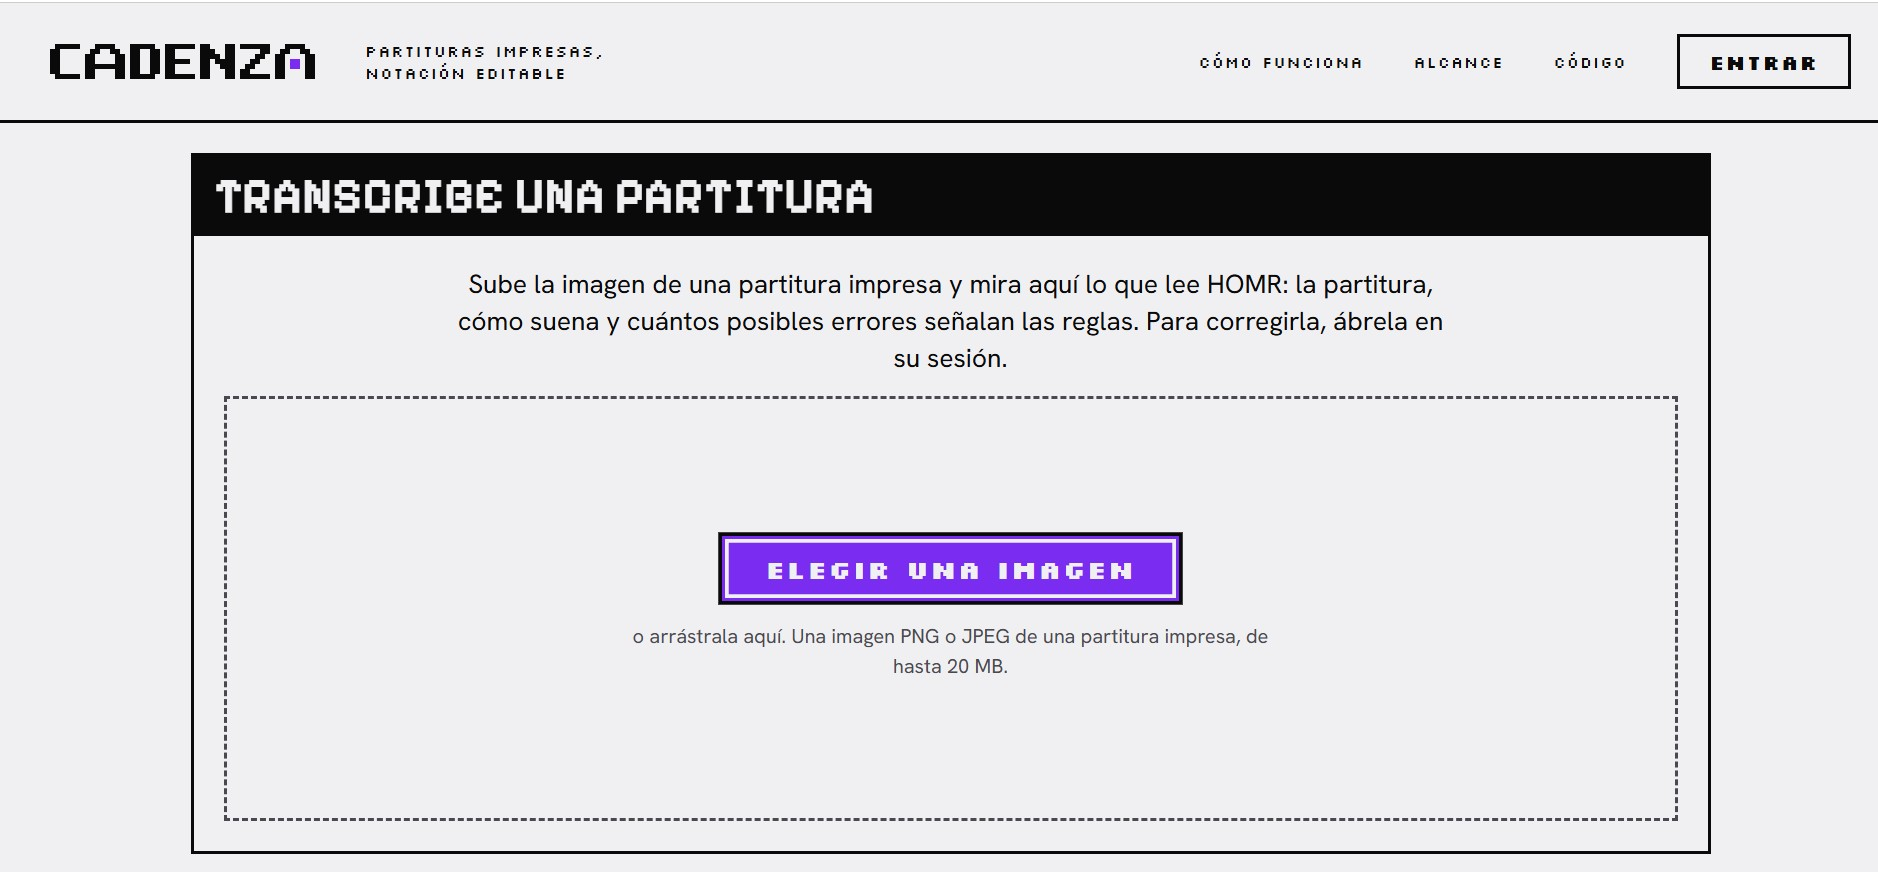
\includegraphics[width=\columnwidth]{portada.jpg}
    \caption{Portada de Cadenza, con la zona para elegir la imagen de una partitura.}
    \label{fig:portada}
\end{figure}

El registro (Figura~\ref{fig:registro}) solo pide un nombre de usuario,
que puede ser un seudónimo, y una contraseña; la plataforma no pide nombre
real ni correo electrónico, y por eso no ofrece recuperación de la
contraseña. El formulario explica qué datos se guardan y con qué fin, y
exige aceptar el permiso de uso de los datos, cuya versión y fecha quedan
en la cuenta.
% fuente: docs/adr/ADR-0012:36-38; docs/adr/ADR-0065:14,23-25
La entrada (Figura~\ref{fig:entrada}) se autentica con un testigo firmado
por el servidor que caduca a los 30 minutos; las contraseñas se guardan
con Argon2id y los intentos de acceso y de registro están limitados por
visitante. Todas las cuentas son iguales y cada una ve solo sus sesiones.
% fuente: docs/adr/ADR-0012:45-53; docs/infra/operacion_backend.md:15,22-26,89; ADR-0070:22-24

\begin{figure}[htbp]
    \centering
    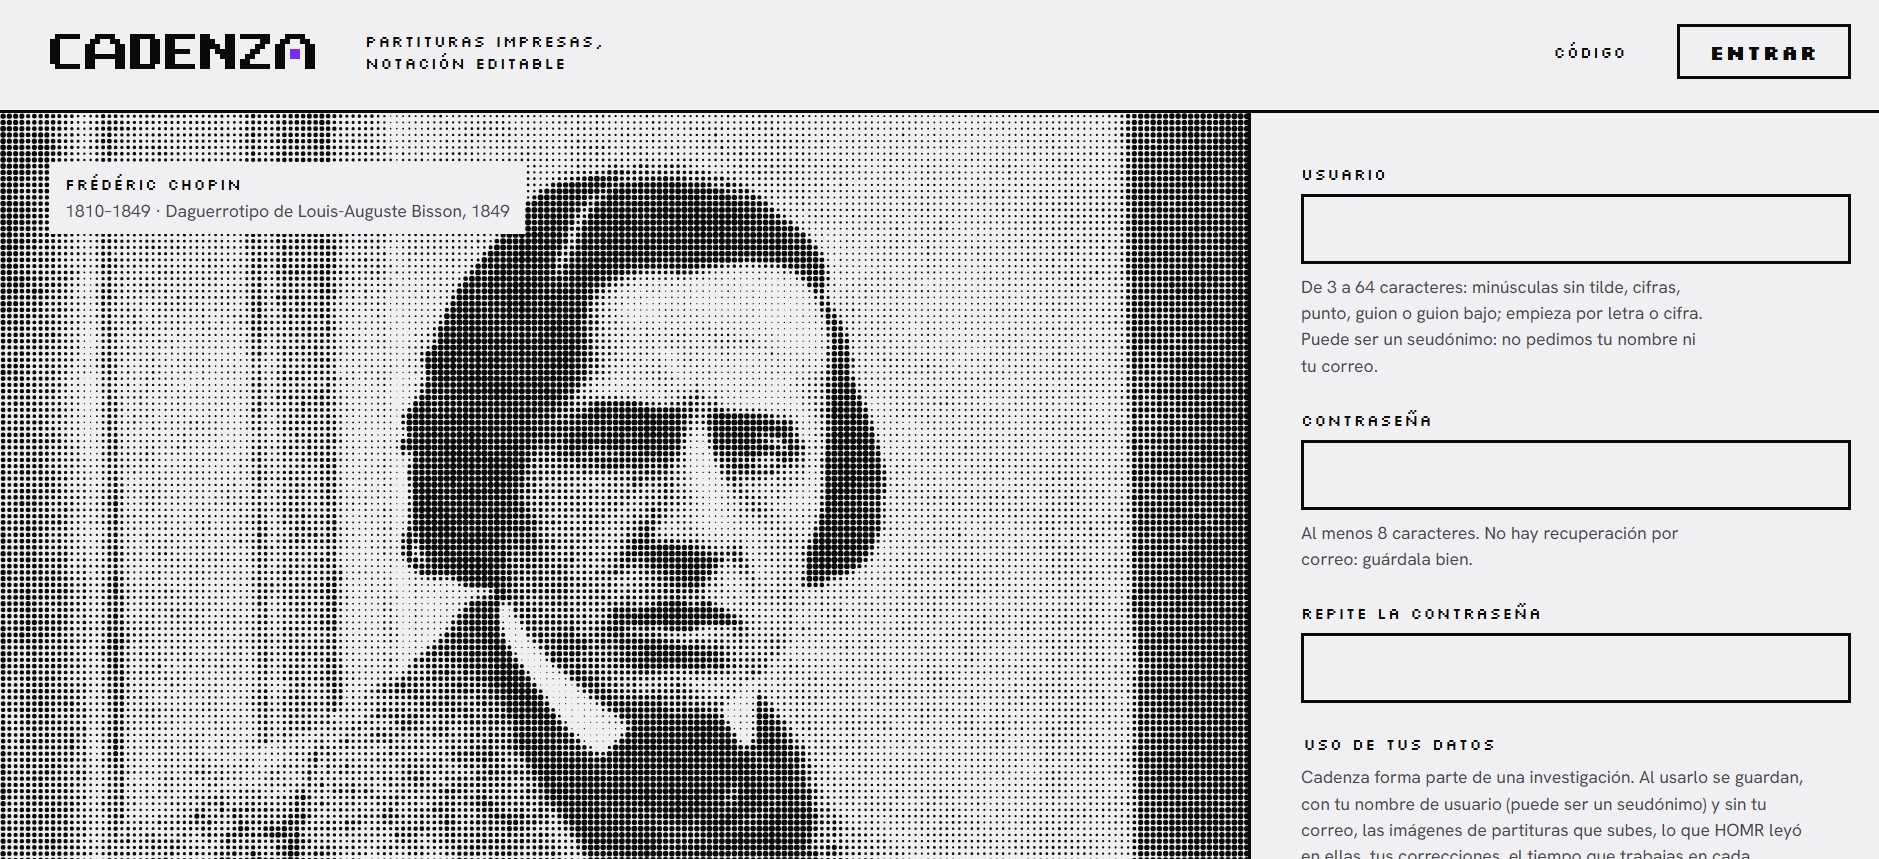
\includegraphics[width=\columnwidth]{registro.jpg}
    \caption{Formulario de registro, con la explicación del uso de los datos.}
    \label{fig:registro}
\end{figure}

\begin{figure}[htbp]
    \centering
    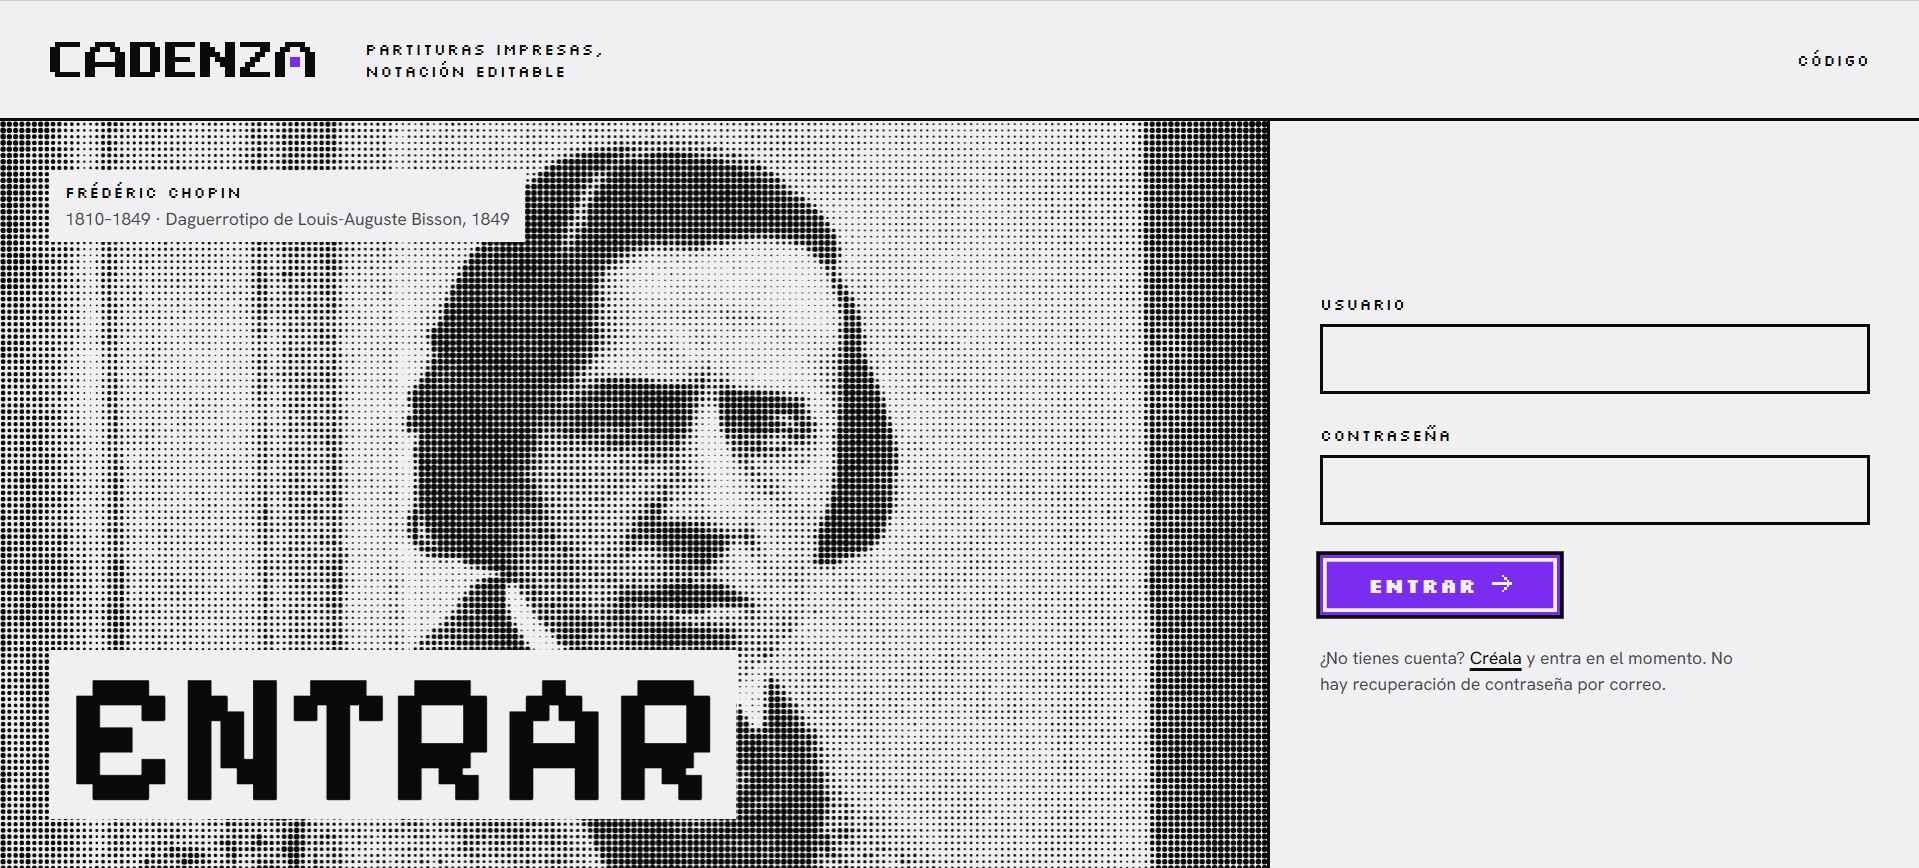
\includegraphics[width=\columnwidth]{entrada.jpg}
    \caption{Formulario de entrada.}
    \label{fig:entrada}
\end{figure}

La transcripción comienza con la carga de una o varias imágenes PNG o JPEG
de hasta 20~MB. Cada imagen entra en una cola que la transcribe en segundo
plano mientras la interfaz informa de su avance, de modo que la lectura de
HOMR, que corre en la GPU del servidor, no bloquea el uso de la
plataforma.
% fuente: README.md:33,157; ADR-0064; ADR-0066
El resultado se importa a la representación simbólica interna, el motor de
validación la analiza y los posibles errores quedan registrados como
hallazgos de la sesión, junto con la imagen original y la captura de lo
que leyó HOMR.

\subsection{Gestión de sesiones}
\label{subsec:sesiones}

Cada transcripción constituye una sesión. El listado
(Figura~\ref{fig:sesiones}) agrupa las sesiones por día, de la más
reciente a la más antigua, y muestra de cada una la miniatura de la
imagen, su título, la hora, el número de posibles errores y su estado:
transcrita, en corrección, finalizada o fallida. Las sesiones pueden
renombrarse y completarse con el compositor y el instrumento de cada
parte.
% fuente: apps/web/src/pages/transcription/days.ts:4-6; SessionPlate.tsx:18-44; sessions.ts:210-213; ADR-0041

% PENDIENTE (captura por rehacer): sesiones.jpg muestra un nombre de usuario que parece real y la etiqueta de rol «Transcriptor», retirada con ADR-0070; además deja ver la dirección de una sesión en la barra de estado del navegador.
\begin{figure}[htbp]
    \centering
    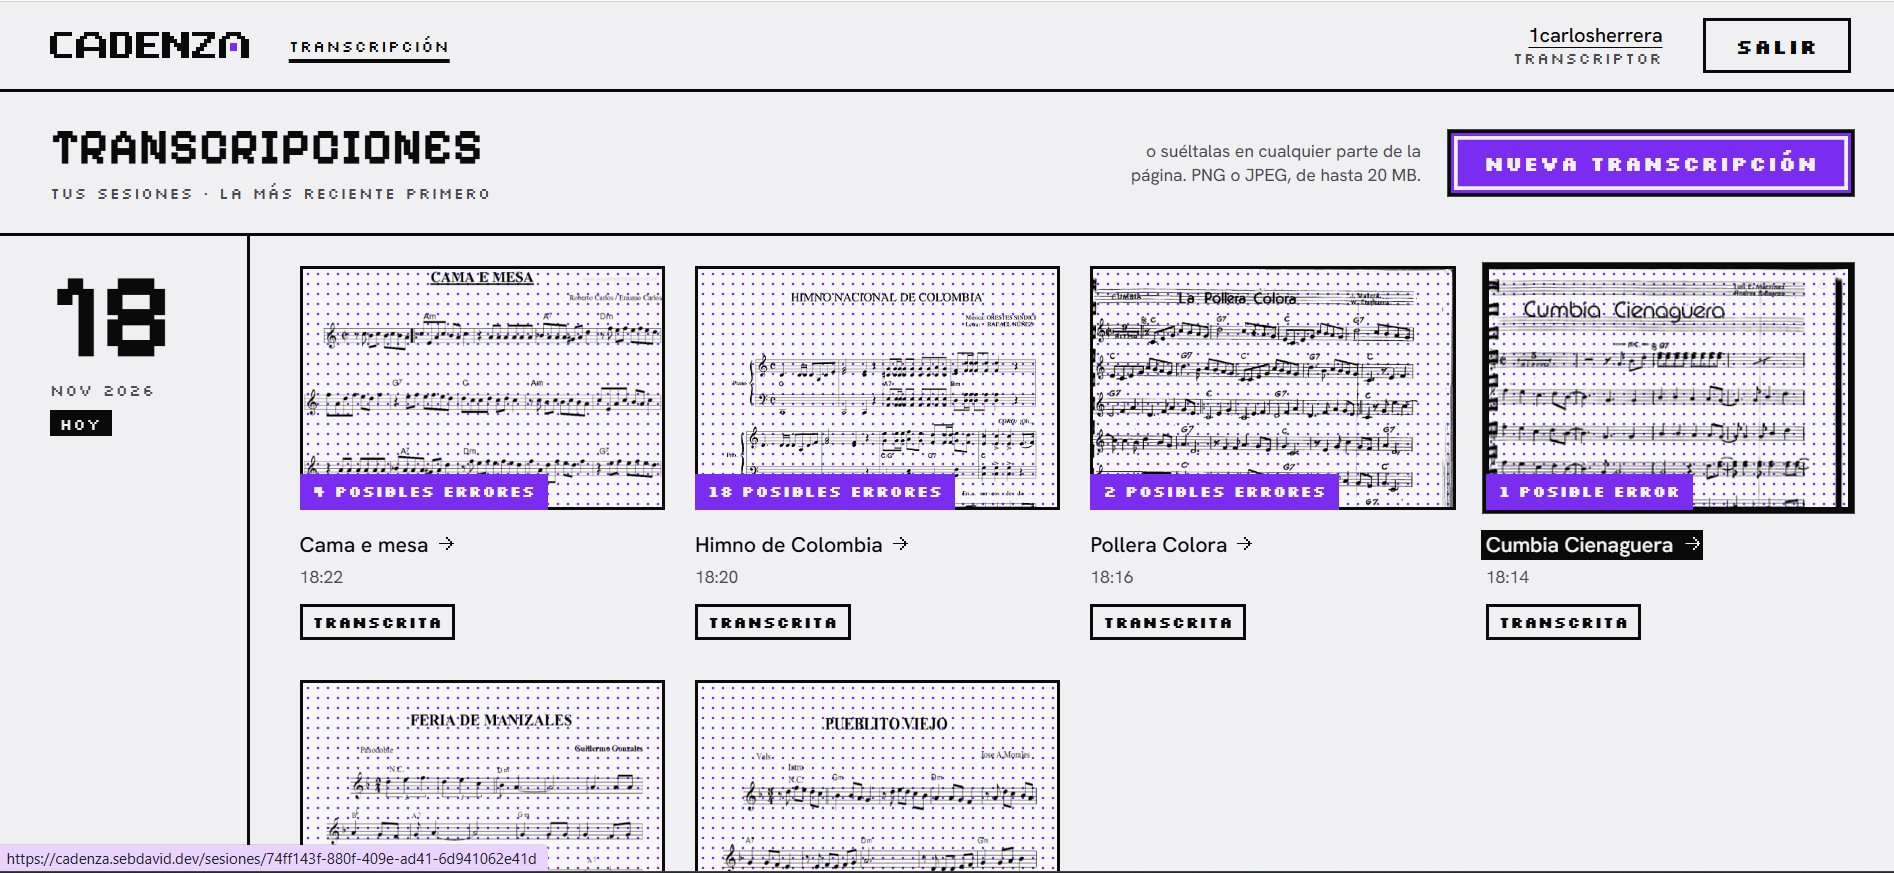
\includegraphics[width=\columnwidth]{sesiones.jpg}
    \caption{Listado de sesiones, agrupadas por día.}
    \label{fig:sesiones}
\end{figure}

\subsection{Vista de corrección asistida}
\label{subsec:vista}

La vista de una sesión (Figura~\ref{fig:vista_sesion}) materializa el
enfoque \textit{Human-in-the-Loop}~\cite{amershi2014}. A la izquierda se
muestra la imagen original, con controles de ampliación y de ajuste al
ancho o a la página; a la derecha, la partitura transcrita. Los compases
en los que las reglas detectaron un posible error aparecen resaltados y
numerados sobre la notación, y un panel lateral los enumera con una
explicación en lenguaje musical. Así, el usuario concentra la revisión en
los puntos sospechosos en lugar de recorrer la partitura símbolo por
símbolo. Cada posible error puede descartarse, si el usuario considera que
no lo es, o restaurarse, y la partitura puede revalidarse después de
corregirla.
% fuente: docs/phases/phase_8_web_interface/README.md:69; README.md:53

% PENDIENTE (captura por rehacer): vista_sesion.jpg, edicion.jpg y exportacion.jpg muestran el mismo nombre de usuario, la etiqueta «Transcriptor» y una partitura con aviso de derechos de autor; vista_sesion.jpg incluye además el borde de las pestañas del navegador.
\begin{figure}[htbp]
    \centering
    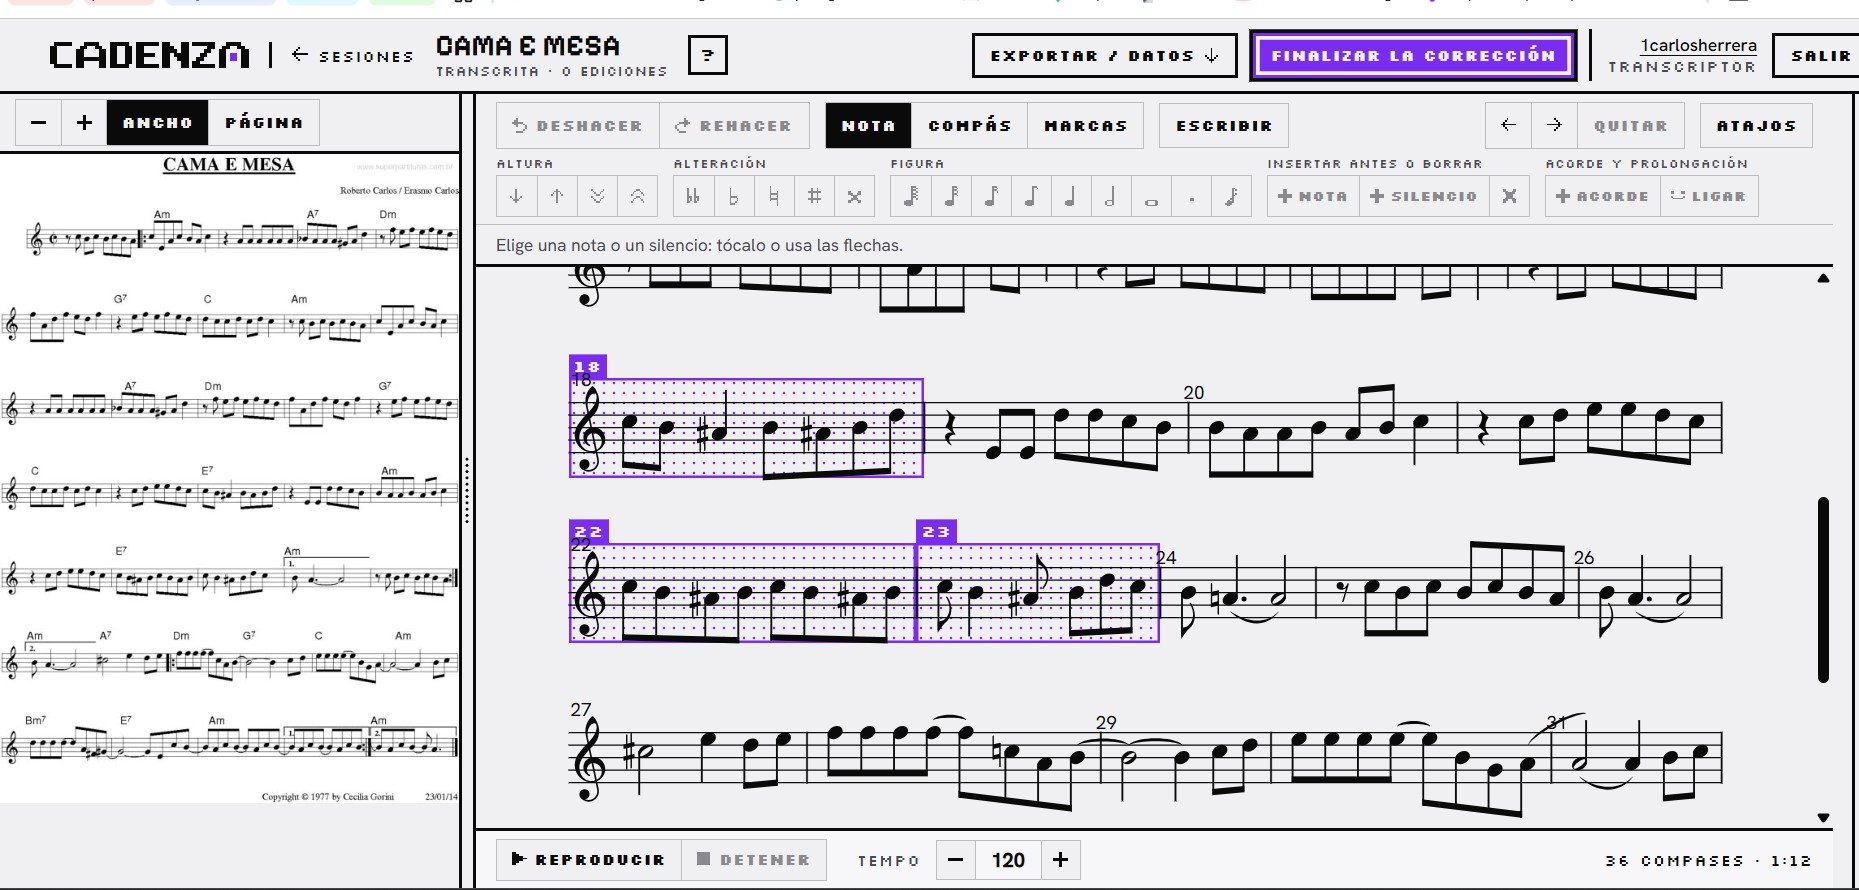
\includegraphics[width=\columnwidth]{vista_sesion.jpg}
    \caption{Vista de una sesión: la imagen original a la izquierda y la partitura transcrita a la derecha, con los compases señalados por las reglas.}
    \label{fig:vista_sesion}
\end{figure}

La corrección se hace directamente sobre la partitura con una barra de
edición de tres pestañas. En la pestaña \textit{Nota}
(Figura~\ref{fig:edicion}), el usuario elige un evento con el ratón o con
las flechas del teclado, y la barra indica su compás, su voz, su altura y
su figura. Desde ella puede cambiar la altura por pasos u octavas, aplicar
alteraciones, cambiar la figura (de semifusa a redonda, con puntillo y
tresillos), insertar o borrar notas y silencios, formar acordes y añadir
ligaduras de prolongación. La pestaña \textit{Compás} permite cambiar la
clave, la armadura y la indicación de compás, y la pestaña
\textit{Marcas}, añadir articulaciones, calderones, dinámicas, ligaduras
de expresión y reguladores. Un modo aparte, \textit{Escribir}, permite
introducir notas con el ratón sobre el pentagrama. Todas las acciones
tienen atajo de teclado.
% fuente: apps/web/src/pages/session/EditBar.tsx:52-58,388,984-990; ADR-0061; README.md:43-51

\begin{figure}[htbp]
    \centering
    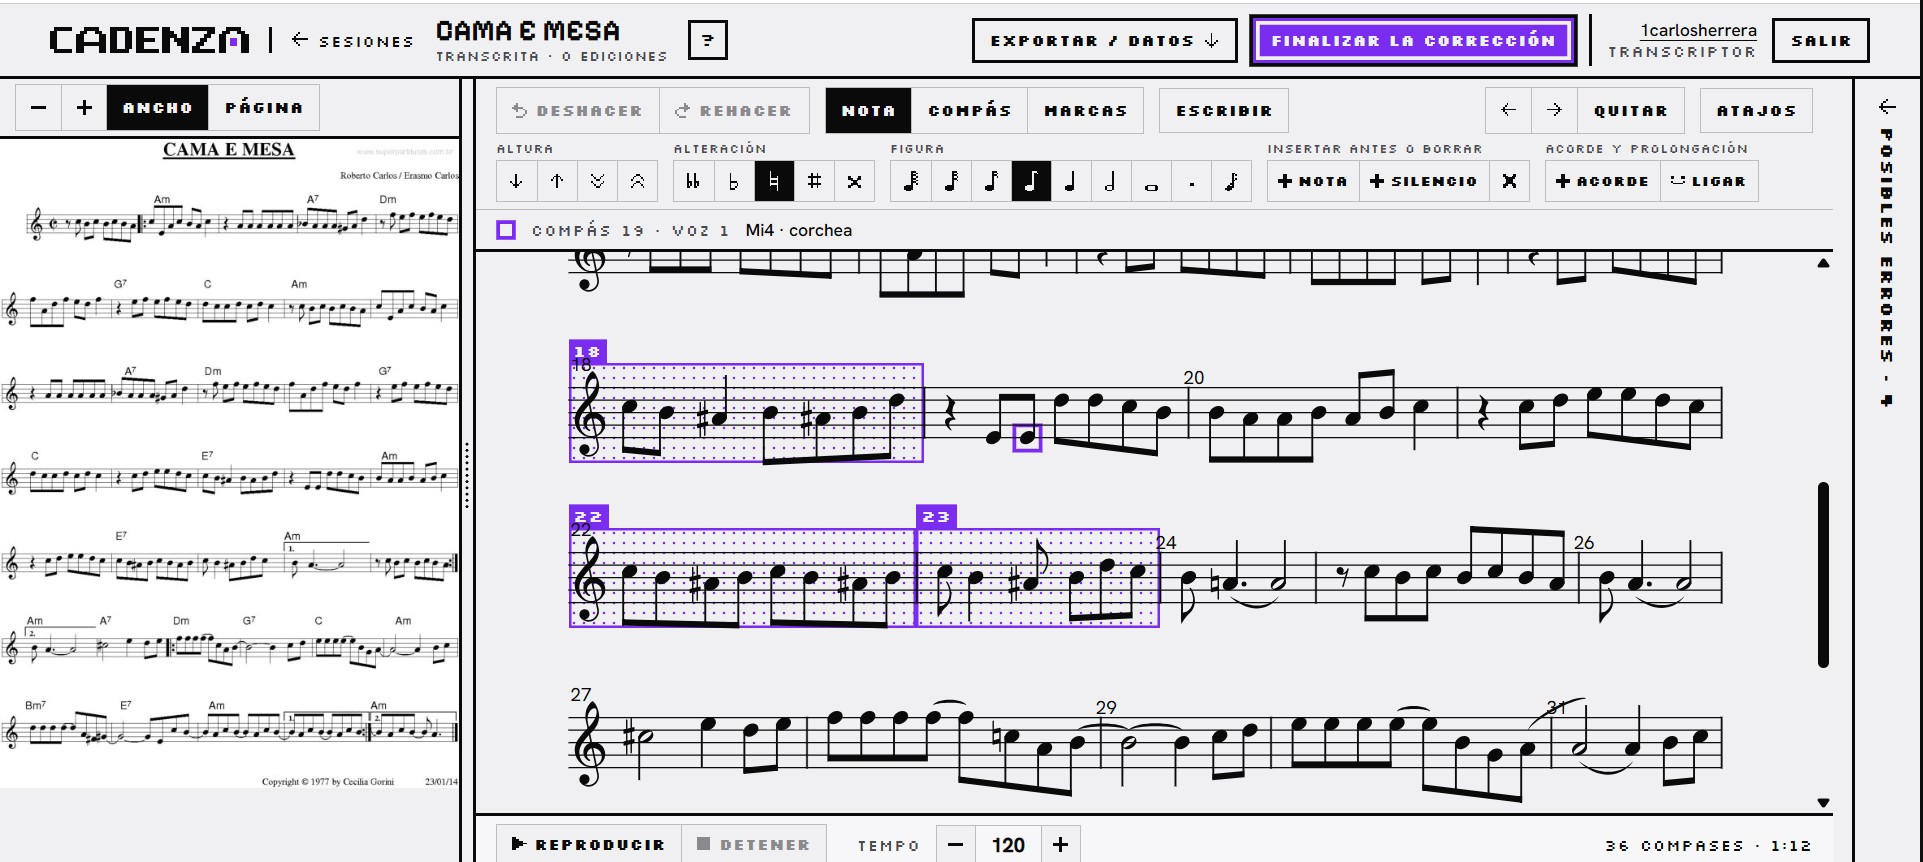
\includegraphics[width=\columnwidth]{edicion.jpg}
    \caption{Edición de una nota: la barra indica el compás, la voz, la altura y la figura del evento elegido.}
    \label{fig:edicion}
\end{figure}

Cada corrección se envía al servidor como una edición atómica, que se
valida antes de guardarse y se añade al registro de la sesión con el
número de secuencia sobre el que se hizo y el autor que fija el servidor.
Deshacer y rehacer actúan sobre ese registro. El estado corregido nunca se
sobrescribe: se reconstruye aplicando el registro al documento original,
lo que conserva la trazabilidad completa entre la salida de HOMR y la
corrección humana.

\subsection{Sugerencias aprendidas}
\label{subsec:sugerencias}

La detección de posibles errores y las sugerencias son dos funciones
distintas. Los posibles errores los señalan las reglas de teoría musical,
siempre. Las sugerencias las propone la capa aprendida, que actúa después:
para un posible error ya señalado, ofrece el arreglo concreto.

Cuando la capa tiene una sugerencia, el posible error del panel la muestra
debajo, con la explicación en lenguaje musical, la confianza expresada en
palabras y dos acciones: aplicar, que registra una edición enlazada a la
sugerencia, y rechazar, que deja el posible error activo. La política de la capa limita lo que se muestra a
las sugerencias de alteración de confianza alta.
% fuente: docs/adr/ADR-0047:19-30; docs/adr/ADR-0036:144-150; issue #258
% fuente: servidor de producción, consulta de solo lectura del 2026-11-19: CADENZA_SUGGESTIONS_ENABLED=true, MIN_LEVEL=high, FAMILIES=accidental; versión promovida sug-estudio-20261103 (frequency_backoff, 2026-11-03). El repositorio (README.md:88, D68) lo da aún por apagado: está desactualizado.

\subsection{Reproducción, finalización y exportación}
\label{subsec:exportacion}

La partitura puede escucharse en cualquier momento, con control del tempo
y con el compás que suena resaltado, lo que permite comprobar de oído la
transcripción. Al terminar, el usuario finaliza la corrección, y la sesión
puede reabrirse si hace falta. El menú \textit{Exportar}
(Figura~\ref{fig:exportacion}) permite cambiar los datos de la sesión y
descargar la partitura corregida en MusicXML~4.0, para editarla en otros
programas; en MIDI~1.0, para reproducirla y sintetizarla; y en PDF, para
imprimirla.
% fuente: ADR-0026:40,58; ADR-0043; ADR-0063; docs/ARCHITECTURE.md:590-592

\begin{figure}[htbp]
    \centering
    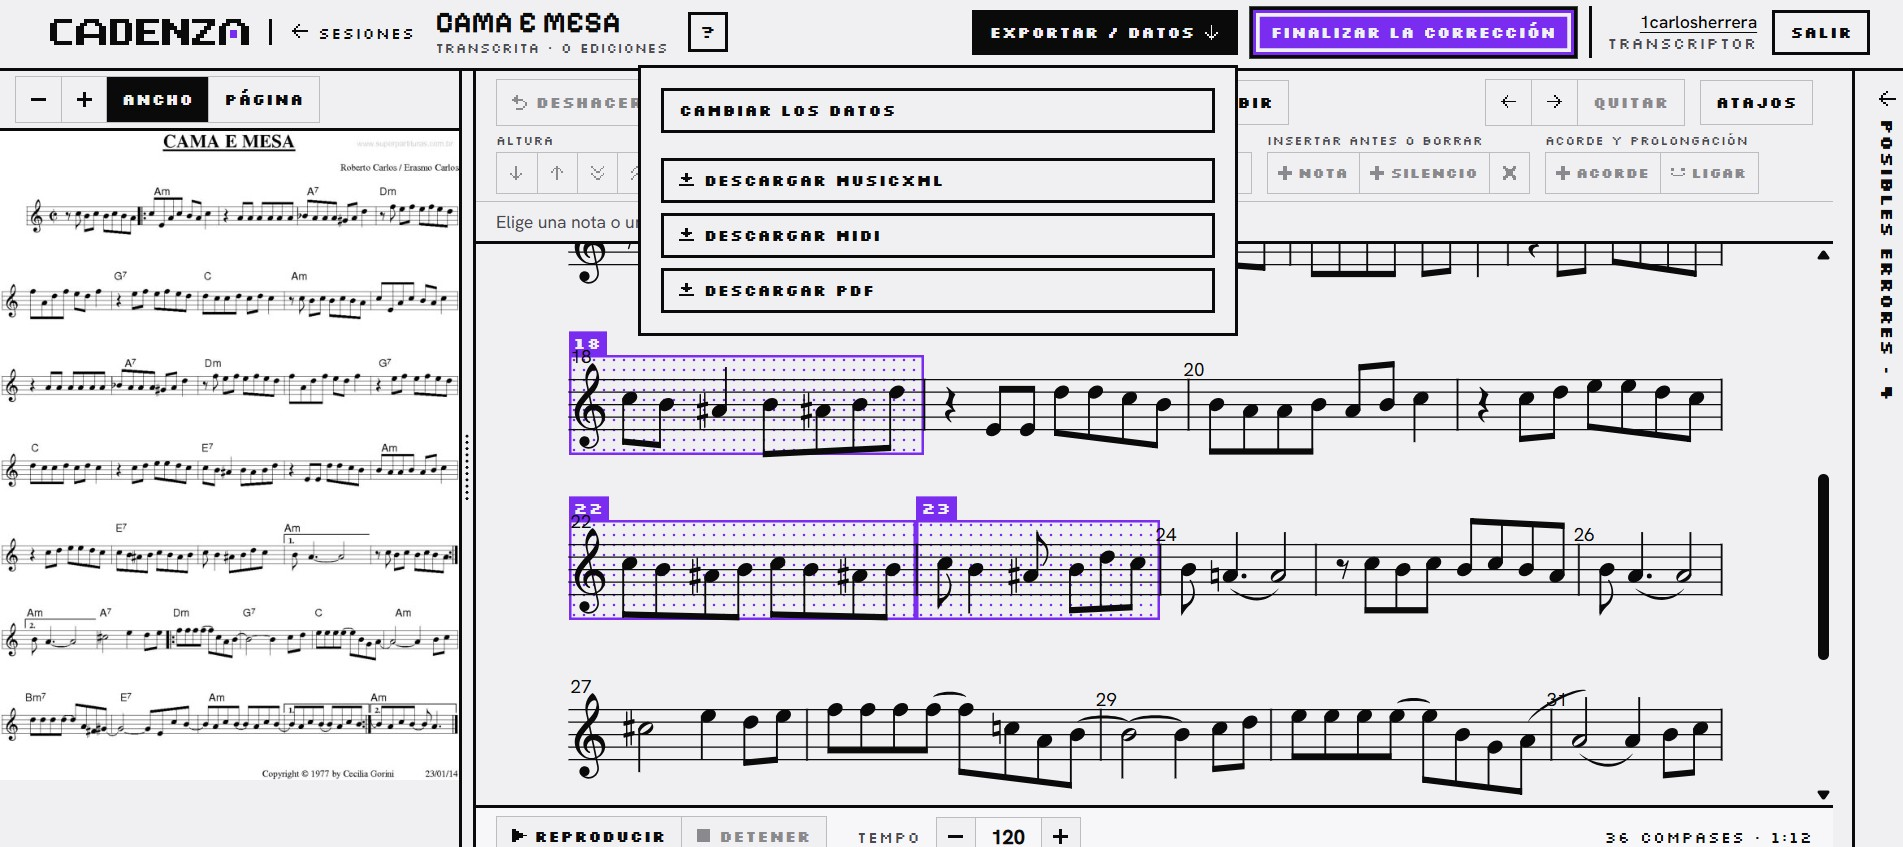
\includegraphics[width=\columnwidth]{exportacion.jpg}
    \caption{Menú de exportación: MusicXML, MIDI y PDF.}
    \label{fig:exportacion}
\end{figure}

\subsection{Datos generados durante el uso}
\label{subsec:datos_uso}

Además de producir la partitura digital, cada sesión genera los datos con
los que la plataforma aprende. Mientras la vista está abierta y visible,
mide el tiempo activo de corrección y el tiempo hasta la primera edición,
descontando las pausas prolongadas; el servidor recuenta las
intervenciones por compás a partir del registro, así como los posibles
errores descartados y restaurados.
% fuente: docs/adr/ADR-0050:16-18,51-53
Cada sesión conserva también el par formado por lo que leyó HOMR y la
versión corregida, que el plano \textit{offline} usa para construir el
corpus de correcciones y exportar los pares de imagen y partitura, siempre
bajo la regla del permiso de uso (Sección~\ref{subsec:datos-lector}). Los
resultados de la capa de sugerencias de este informe se miden sobre un
corpus de referencia y no sobre correcciones humanas.

\subsection{Página de los errores del reconocedor}
\label{subsec:pagina-errores}

El prototipo incluye una página, accesible sin cuenta, que muestra qué
notas lee mal HOMR y cómo se corrigen. Presenta las cifras por origen: las
de los corpus PrIMuS y Camera-PrIMuS, donde la corrección es la partitura
de referencia, y las de las transcripciones terminadas en Cadenza, que solo
aparecen como cifras de conjunto y cuando reúnen el mínimo de sesiones y de
cuentas descrito en la Sección~\ref{sec:arquitectura}. La página se
actualiza sola.
% fuente: apps/web/src/pages/homr-errors/ (ruta /errores-de-homr, apps/web/src/router.tsx:24); docs/adr/ADR-0073; issues #423, #424 y #449

La cabecera resume lo más relevante y da los totales
(Figura~\ref{fig:errores-cifras}). Para el corpus de PrIMuS, HOMR leyó
33\,115 notas y silencios en 1\,877 íncipits; el 86\,\% quedó igual que
en la referencia, 3\,986 hubo que corregirlos, 660 sobraban y 739 no se
leyeron. Cada lectura se compara con la referencia en orden, de principio a
fin, y no compás por compás: si HOMR no leyó una barra de compás, las notas
de los dos lados siguen contando como bien leídas y el error se registra
como barra no leída (89 en PrIMuS, y 5 barras de más). Estos totales cuentan todos los íncipits leídos, y no solo
aquellos cuya secuencia de correcciones se verifica, que son los de la
Tabla~\ref{tab:tipos-error}.
% fuente: /errores-de-homr, grupo «primus» (1877 íncipits, 33.115 leídos, 86 % bien, 3986 corregidos, 660 sobraban, 739 no leídos; 89 barras no leídas y 5 de más), consultado el 2026-11-19 tras desplegar 44b1741 y copiar el corpus de exp_12 regenerado con el formato 2 (#466, ADR-0075: alineación del íncipit entero). Antes, con la alineación compás a compás: 84,9 %, 3966, 1032 y 835.

\begin{figure*}[!t]
    \centering
    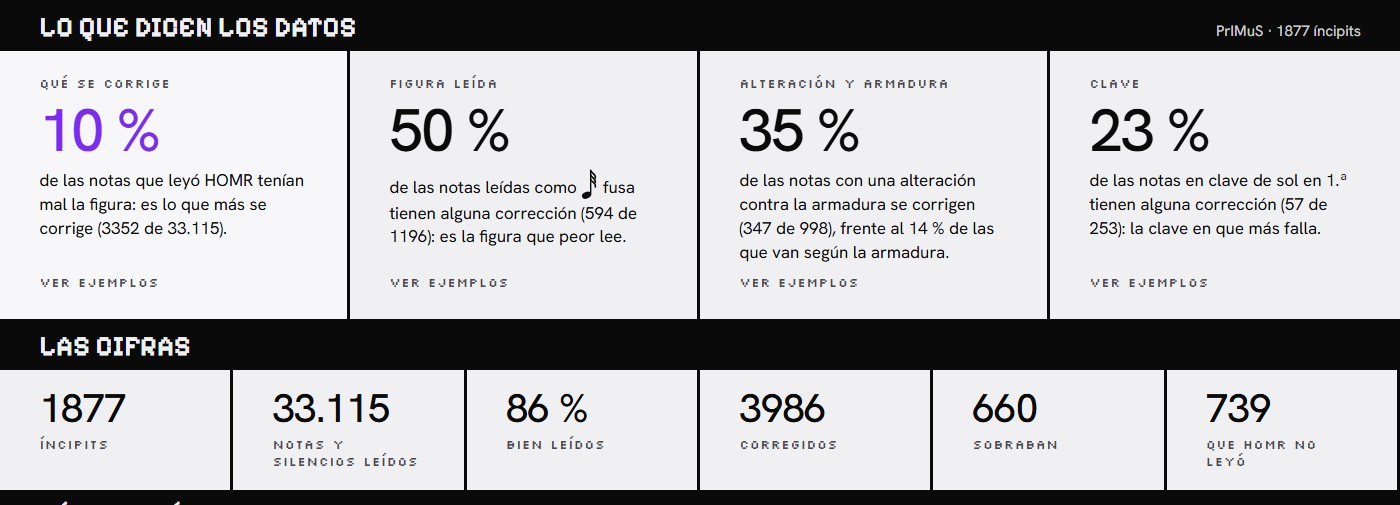
\includegraphics[width=\textwidth]{errores_cifras.jpg}
    \caption{Página de los errores del reconocedor: resumen y totales del corpus de PrIMuS.}
    \label{fig:errores-cifras}
\end{figure*}

El cuerpo de la página (Figura~\ref{fig:errores-detalle}) responde a
cuatro preguntas: qué pasó con cada nota leída, qué se corrige por cada
cien notas, cuánto se desplazó la altura en las correcciones de altura y
dónde se equivoca más el reconocedor, según la alteración frente a la
armadura, la clave y la figura leída. Cada cifra lleva a ejemplos del
corpus: la imagen del íncipit y, debajo, el compás dibujado dos veces, tal
como lo leyó HOMR y tal como es, con la nota del ejemplo resaltada. Un
historial permite buscar cualquier partitura del corpus y ver sus
correcciones.

\begin{figure*}[!t]
    \centering
    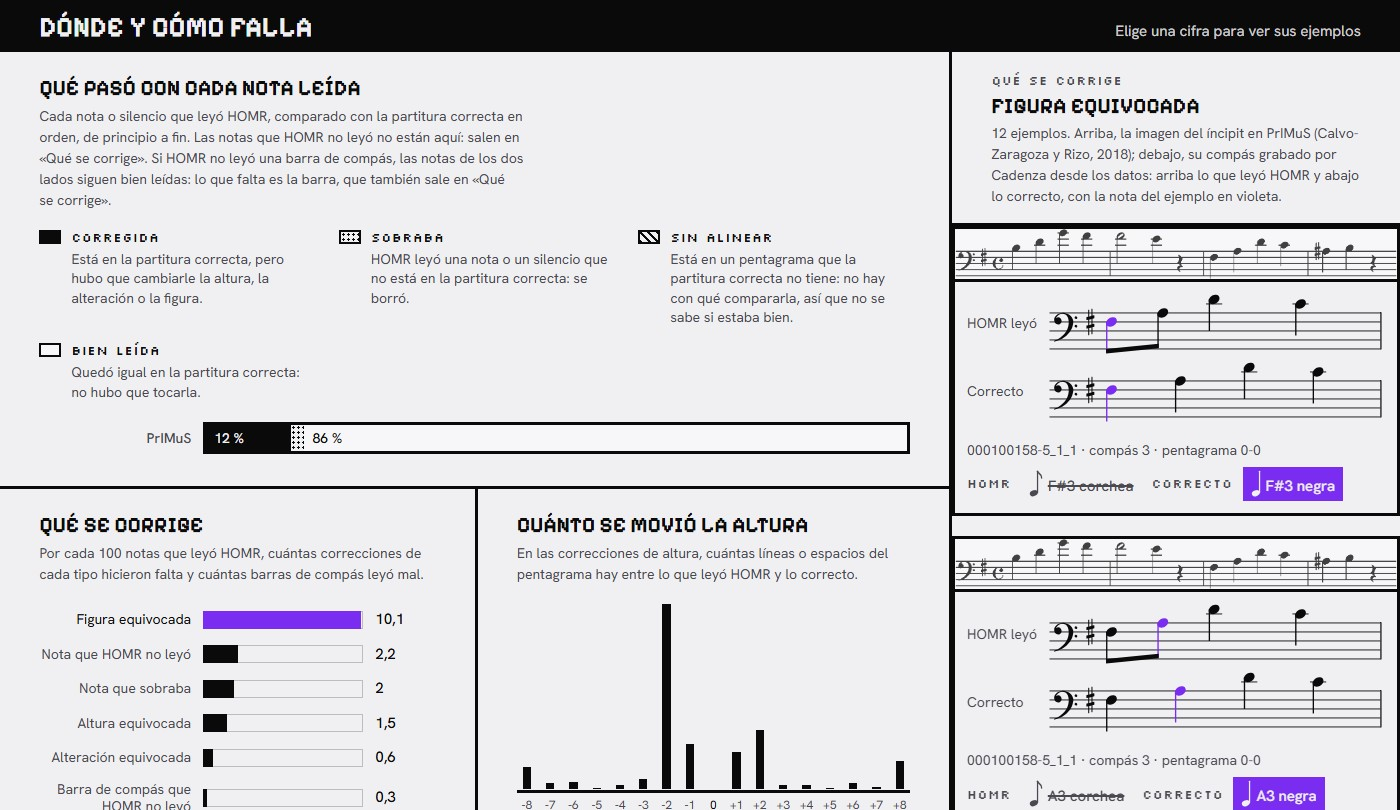
\includegraphics[width=\textwidth]{errores_detalle.jpg}
    \caption{Página de los errores del reconocedor: qué pasó con cada nota, qué se corrige y cuánto se desplazó la altura; a la derecha, ejemplos con la imagen del íncipit y el compás como lo leyó HOMR y como es.}
    \label{fig:errores-detalle}
\end{figure*}

La matriz de la Figura~\ref{fig:errores-figuras} cruza la figura que leyó
HOMR con la que era. Hace visible el patrón que domina los errores: el
reconocedor lee una figura de la mitad de duración, y la casilla más
frecuente, con 1\,700 casos, es la corchea leída donde había una negra. De
ejemplos con fotografías de usuarios no se muestra ninguno: de las
sesiones de Cadenza solo salen cifras.
% fuente: GET /api/stats/homr-errors, grupo «primus», durations (corchea leída, negra correcta: 1700); captura de la página del 2026-11-19

\begin{figure}[htbp]
    \centering
    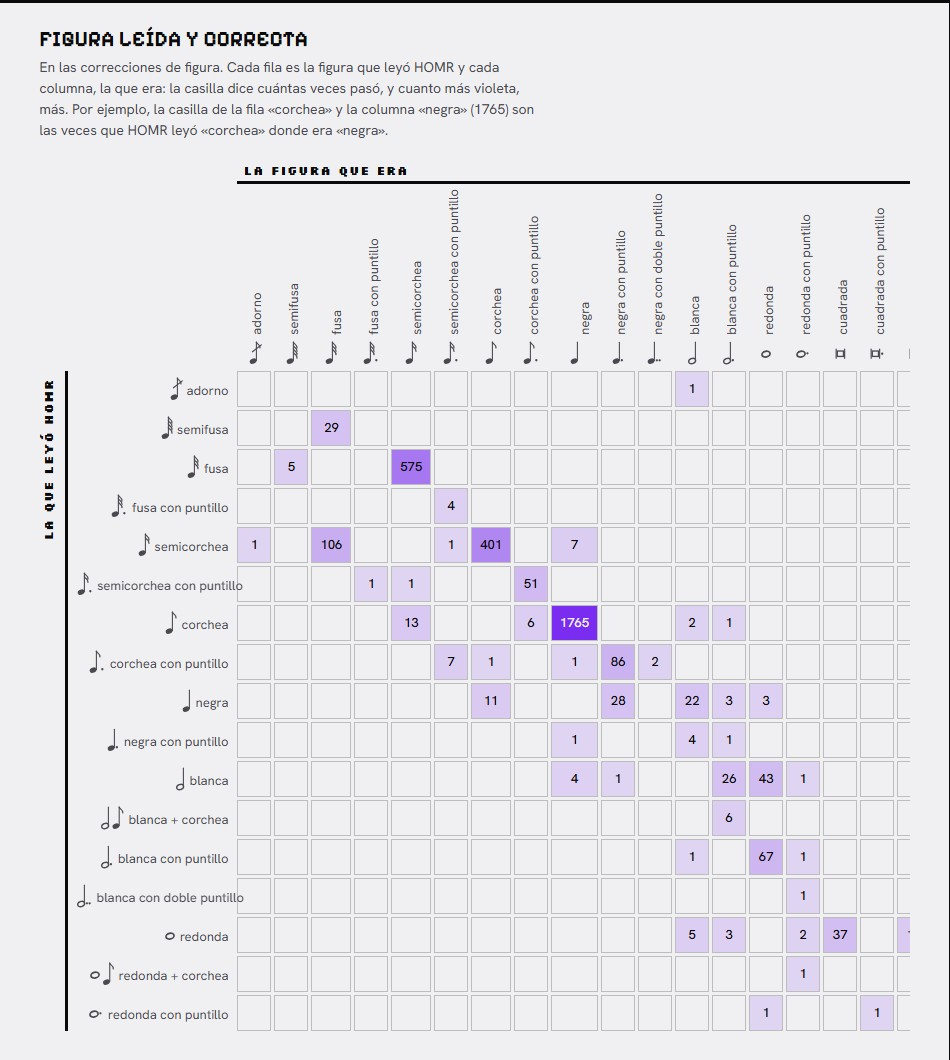
\includegraphics[width=\columnwidth]{errores_figuras.jpg}
    \caption{Figura leída por HOMR frente a la figura correcta en las correcciones de figura del corpus de PrIMuS.}
    \label{fig:errores-figuras}
\end{figure}

% ============================================================================
% IX. RESULTADOS
% Regla del proyecto (CLAUDE.md §8): toda cifra sale de un archivo medido de
% results/ («simulated»: false) o de un documento del repositorio.
% Nota: las cifras son las de los archivos de results/ tal como estaban el
% 2026-11-19, comprobadas una a una contra los JSON. Por decisión del
% responsable no se vuelven a ejecutar los experimentos para este informe.
% results/ no está versionado en git.
% ============================================================================

\section{Resultados}
\label{sec:resultados}

Esta sección reúne las mediciones del proyecto. Todas proceden de
ejecuciones reales del motor sobre conjuntos de datos con verdad de
referencia, y ninguna es simulada. No incluye mediciones con personas: el
estudio con participantes quedó fuera del alcance. Las métricas de fidelidad son la tasa de
error simbólico (SER) y la distancia de edición normalizada
OMR-NED~\cite{smb2025}; en ambas, un valor menor es mejor.

\subsection{Calidad del reconocimiento}

La Tabla~\ref{tab:calidad-omr} resume la calidad de HOMR~0.7.0 sobre tres
muestras de íncipits monofónicos impresos: dos de
PrIMuS~\cite{calvo2018} y una de Camera-PrIMuS~\cite{cameraprimus2018},
cuyas imágenes llevan distorsiones que simulan una fotografía. En todos
los casos, el fallo de lectura consiste en que el motor no encuentra
pentagramas en la imagen.

% fuente (fila 1): results/omr_baseline_summary.json (total_evaluated 100, failures_count 9, metrics_on_successes.mean_ser 0.1124, .mean_omr_ned 0.2341); results/exp_03_run_info.json
% fuente (fila 2): results/correction_corpus_summary.json (sample.size 2000, transcription.transcribed 1878, .failure_rate 0.061, omr_ned.mean 0.2344 sobre 1877); SER: results/exp_15_compas/reference_set_summary.json:primus[1].omr_quality.ser.mean_before 0.1339 (n 1877); results/exp_12_run_info.json (homr 0.7.0, cpu)
% fuente (fila 3): results/camera_primus_correction_corpus_summary.json (sample.size 3000, transcription.transcribed 2242, .failure_rate 0.2527, ser.mean 0.193, omr_ned.mean 0.3333); results/exp_18_run_info.json (simulated false, homr 0.7.0, cuda)
\begin{table}[htbp]
\caption{Calidad de HOMR 0.7.0 sobre íncipits impresos}
\label{tab:calidad-omr}
\centering
\footnotesize
\setlength{\tabcolsep}{3pt}
\begin{tabular}{|p{2.35cm}|c|c|c|c|c|}
\hline
\textbf{Muestra} & \textbf{N} & \textbf{Leídos} & \textbf{Fallos} & \textbf{SER} & \textbf{NED} \\
\hline
PrIMuS, línea base & 100 & 91 & 9,0\,\% & 0,112 & 0,234 \\
\hline
PrIMuS, corpus & 2\,000 & 1\,878 & 6,1\,\% & 0,134 & 0,234 \\
\hline
Camera-PrIMuS & 3\,000 & 2\,242 & 25,3\,\% & 0,193 & 0,333 \\
\hline
\multicolumn{6}{|p{7.6cm}|}{\scriptsize SER y OMR-NED (NED): medias sobre los íncipits leídos, sin penalizar los fallos. En el corpus de PrIMuS, las métricas se calculan sobre 1\,877 íncipits, porque una referencia no pudo leerse.} \\
\hline
\end{tabular}
\end{table}

En la línea base, la mediana de la SER es 0,039, muy por debajo de la
media, lo que indica que la mayoría de los íncipits se lee con pocos
errores y que unos pocos concentran el error. Si los nueve fallos de
lectura se cuentan como error total, la SER media sube a 0,192 y el
OMR-NED medio a 0,303.
% fuente: results/omr_baseline_summary.json (metrics_on_successes.median_ser 0.0385; metrics_penalized_with_failures.mean_ser_penalized 0.1923, .mean_omr_ned_penalized 0.303)
Las tres muestras se midieron en fechas y con dispositivos distintos, por
lo que la tabla describe cada una y no constituye una comparación
controlada entre ellas.
% fuente: docs/PROJECT_STATE.md:412 («Las comparaciones con exp_12 no se citan»)

\subsection{Errores del reconocedor}

Para saber qué corrige una persona cuando revisa una lectura de HOMR, se
derivó la secuencia de ediciones que lleva de cada lectura a su verdad de
referencia y se conservaron solo las secuencias verificadas, es decir,
aquellas que al aplicarse reproducen la referencia. En el corpus de PrIMuS
se verificó el 96,9\,\% de los íncipits leídos (1\,818 de 1\,877), con
4\,994 correcciones, 2,75 de media por íncipit; en la muestra de
Camera-PrIMuS, el 68,8\,\% (1\,543 de 2\,242), con 4\,549 correcciones.
% fuente: results/correction_corpus_summary.json (verification.verified_count 1818, .rate 0.9686; edit_distribution.verified.counts.Total 4994; average_edits_per_verified_incipit 2.75); results/camera_primus_correction_corpus_summary.json (verification.verified_count 1543, .rate 0.6882; Total 4549; regenerado el 2026-11-19 con 44b1741)
La Tabla~\ref{tab:tipos-error} muestra cómo se reparten por tipo.

% fuente: results/correction_corpus_summary.json:edit_distribution.verified.proportions (SetDuration 0.6231, InsertEvent 0.1288, DeleteEvent 0.1217, SetPitch 0.0849, SetAccidental 0.0402, SetClef 0.0008, SetKey 0.0004)
% fuente: results/camera_primus_correction_corpus_summary.json:edit_distribution.verified.proportions (SetDuration 0.4346, InsertEvent 0.1545, DeleteEvent 0.1392, SetPitch 0.1699, SetAccidental 0.0785, SetClef 0.0075, SetKey 0.0158)
\begin{table}[htbp]
\caption{Correcciones verificadas por tipo}
\label{tab:tipos-error}
\centering
\footnotesize
\begin{tabular}{|l|c|c|}
\hline
\textbf{Tipo de corrección} & \textbf{PrIMuS} & \textbf{Camera-PrIMuS} \\
\hline
Cambiar la figura & 62,3\,\% & 43,5\,\% \\
\hline
Insertar un evento & 12,9\,\% & 15,5\,\% \\
\hline
Borrar un evento & 12,2\,\% & 13,9\,\% \\
\hline
Cambiar la altura & 8,5\,\% & 17,0\,\% \\
\hline
Cambiar la alteración & 4,0\,\% & 7,8\,\% \\
\hline
Cambiar la armadura & 0,04\,\% & 1,6\,\% \\
\hline
Cambiar la clave & 0,08\,\% & 0,7\,\% \\
\hline
\textbf{Correcciones} & \textbf{4\,994} & \textbf{4\,549} \\
\hline
\end{tabular}
\end{table}

En ambas muestras domina el error de figura. Buena parte de él procede de
la indicación de compás: HOMR la lee mal en el 37,6\,\% de los íncipits
del corpus de PrIMuS y en el 41,6\,\% de la muestra de Camera-PrIMuS.
% fuente: results/correction_corpus_summary.json:time_signature.incipits_with_time_misread (705/1877, 0.3756); results/camera_primus_correction_corpus_summary.json:time_signature.incipits_with_time_misread (933/2242, 0.4161)
Estas correcciones son las de un corrector ideal, obtenidas por
alineación con la referencia, y no las de una persona; además, las
distorsiones de Camera-PrIMuS son sintéticas y no fotografías reales.
% fuente: docs/adr/ADR-0036:173-177; docs/adr/ADR-0074:36

\subsection{Etapas propias tras la lectura}

A partir de ese diagnóstico se añadió, después de HOMR, una etapa que
corrige la indicación de compás. Sobre 1\,968 íncipits de PrIMuS, el
numerador del compás pasa de ser correcto en el 62,8\,\% a serlo en el
87,3\,\%, y la notación del compás, del 33,5\,\% al 86,1\,\%. La SER media
de los 1\,877 íncipits del corpus baja de 0,134 a 0,097, con 480 íncipits
que mejoran y 13 que empeoran.
% fuente: results/exp_15/reference_set_summary.json:headline.primus (numerator_correct 1236/1968 = 0.628; notation_correct 660/1968 = 0.3354) y results/exp_15_compas/reference_set_summary.json:headline.primus (1717/1968 = 0.8725; 1695/1968 = 0.8613); :primus[1].omr_quality.ser (mean_before 0.1339, mean_after 0.0966, better 480, worse 13); simulated false
La mejora de la SER refleja el mismo acierto del compás, pesado por
compases, y no es una prueba independiente.
% fuente: docs/adr/ADR-0059:88
% PENDIENTE: el OMR-NED de exp_14 y exp_15 no se cita: se midió con un exportador anterior y debe regenerarse (deuda D70, docs/PROJECT_STATE.md:131).

Sobre doce páginas impresas de voz con piano, con verdad de referencia de
una edición abierta, la proporción de pentagramas que la importación deja
en su lugar pasó del 17,2\,\% al 95,5\,\% (701 de 734) con la etapa que
conserva el orden de las partes. Los tresillos sin marca explícita siguen
sin leerse: ninguno de los dos compases del conjunto que los contienen.
% fuente: results/exp_15_voz_y_piano_antes/reference_set_summary.json:headline.pages.staves_in_place (126/734 = 0.1717); results/exp_15_piano_combinado/…:staves_in_place (701/734 = 0.955); results/exp_15_compas/…:tuplet_measures_implicit_read (0/2); ADR-0056 (doce páginas de IMSLP, verdad de OpenScore Lieder)

\subsection{Validación por reglas}

La Tabla~\ref{tab:validacion} recoge el desempeño del catálogo vigente de
reglas, evaluado compás a compás: un compás cuenta como acierto cuando las
reglas lo señalan y contiene al menos un error real de lectura.

% fuente (columna 1): results/rules_catalog_v2/exp_06/validation_metrics_summary.json:global_metrics (tp 74, fp 19, fn 127, tn 139, total 359; precision 0.7957, recall 0.3682, f1 0.5034, accuracy 0.5933, specificity 0.8797)
% fuente (columna 2): results/rules_catalog_v2/exp_14/suggestion_layer_summary.json:test.rule_blind_measures.rules.global_metrics (tp 255, fp 205, fn 174, tn 893, total 1527; precision 0.5543, recall 0.5944, f1 0.5737, accuracy 0.7518, specificity 0.8133)
\begin{table}[htbp]
\caption{Desempeño de las reglas de validación, por compás}
\label{tab:validacion}
\centering
\footnotesize
\begin{tabular}{|l|c|c|}
\hline
\textbf{Medida} & \textbf{91 íncipits} & \textbf{352 íncipits} \\
\hline
Compases & 359 & 1\,527 \\
\hline
Precisión & 0,796 & 0,554 \\
\hline
Sensibilidad & 0,368 & 0,594 \\
\hline
F1 & 0,503 & 0,574 \\
\hline
Exactitud & 0,593 & 0,752 \\
\hline
Especificidad & 0,880 & 0,813 \\
\hline
\multicolumn{3}{|p{6.6cm}|}{\scriptsize Las dos evaluaciones usan definiciones distintas de la verdad de referencia y no son comparables entre sí.} \\
\hline
\end{tabular}
\end{table}

En la primera evaluación, casi cuatro de cada cinco compases señalados
contienen un error real, pero las reglas solo alcanzan algo más de un
tercio de los compases con error. Los falsos positivos esperados
corresponden al último compás, incompleto, de un íncipit cortado. Por
categoría, las reglas cubren el 71,2\,\% de los compases con errores de
duración y el 29,9\,\% de los de alteración.
% fuente: results/rules_catalog_v2/exp_06/validation_metrics_summary.json:coverage_by_category (duration 0.7119, 42/59; accidental 0.2992, 38/127); :coverage_analysis.false_positive_nature

Una simulación anterior, hecha con la primera versión del catálogo,
estimó cuánto se reduce la inspección si el usuario mira solo los
compases señalados: 124 de 359, un 65,5\,\% menos. Esa reducción tiene un
costo que la propia medición declara: el 60,2\,\% de los compases con
error no se señalaba. Es una cuenta de compases por mirar y no una medida
de tiempo de edición.
% fuente: results/effort_comparison.json:inspection_effort (359, 124, effort_reduction_percent 65.46); :error_detection_and_tradeoff.missed_errors_rate 0.602; results/exp_01_run_info.json

\subsection{Capa de sugerencias}

La capa se entrenó con las correcciones de 1\,466 íncipits del corpus de
PrIMuS y se evaluó sobre 352 íncipits de prueba, separados por obra. De
las cinco familias de corrección que modela, solo la de alteraciones
supera el umbral de precisión fijado por validación cruzada y queda
activa.
% fuente: results/rules_catalog_v2/exp_14/suggestion_layer_summary.json (corpus.train.measured_incipits 1466, corpus.test.measured_incipits 352; model.families: accidental activa, duration, pitch, delete e insertion inactivas; simulated false)

El primer resultado es el orden de las sugerencias. En los 79 hallazgos de
la prueba cuyo arreglo verdadero está entre los candidatos, la capa lo
pone en primer lugar en 68 (86,1\,\%), frente a 53 (67,1\,\%) con el orden
que dan las reglas. La validación cruzada de cinco pliegues agrupados por
obra da $0{,}857 \pm 0{,}026$ frente a $0{,}737 \pm 0{,}058$.
% fuente: ídem:test.rule_suggestions (with_true_candidate 79; top1.over_true_candidate 68/79 = 0.8608; baseline_rule_order.top1.over_true_candidate 53/79 = 0.6709); :cross_validation (rule_top1_accuracy 0.8569 / 0.0258; baseline_top1_accuracy 0.7372 / 0.0578)

El segundo es el efecto de la política de la capa, que solo
muestra las sugerencias de alteración de confianza alta. Con ella se
muestran 45 sugerencias, de las cuales 40 son correctas (88,9\,\%). Si se
aplican todas las de confianza alta, 40 de 47 arreglan un error y 3
estropean una nota que estaba bien, y la SER media baja de 0,1334 a
0,1297: mejora en 23 íncipits, empeora en 1 y no cambia en 328.
% fuente: results/rules_catalog_v2/exp_14_politica_alteraciones_alta/suggestion_layer_summary.json:test.rule_suggestions (with_suggestions 45; top1.over_findings_with_suggestions 40/45 = 0.8889); :test.damage.high.applied (suggestions 47, correct 40, damaged_correct_events 3); :before_after.ser (homr 0.1334, homr_with_high 0.1297; improved 23, worsened 1, unchanged 328)
En cambio, aplicar a ciegas la primera sugerencia de cada hallazgo, sin
filtro de confianza, empeora la lectura: la SER media sube a 0,154.
% fuente: results/rules_catalog_v2/exp_14/suggestion_layer_summary.json:before_after.ser.homr_with_first.mean 0.1541

El tercero es un resultado negativo. Con la primera versión del catálogo,
la capa señalaba por sí misma 38 posibles errores de alteración que las
reglas no veían, 33 de ellos correctos. Con el catálogo vigente, que
incorpora una regla para las alteraciones repetidas, ese aporte propio
desaparece: la capa señala 2 posibles errores, ninguno correcto, y no
encuentra ninguno de los 632 errores que las reglas no ven.
% fuente: results/suggestion_layer_summary.json:test.learned_findings (count 38, correct 33) y results/rules_catalog_v2/exp_14/suggestion_layer_summary.json:test.learned_findings (count 2, correct 0), :test.rule_blind_events (errors 632, flagged 0)
El valor medido de la capa está, por tanto, en ordenar mejor los arreglos
de lo que las reglas ya detectan, y no en detectar errores nuevos.

Estas cifras tienen dos salvedades. Las correcciones son las de un
corrector ideal, no las de personas. Y la tasa de aceptación de las
sugerencias por los usuarios no se ha analizado: las respuestas reunidas
son todavía muy pocas para informar de ella.
% fuente: ídem:study_sessions (available false, sessions 0, acceptance_rate null)
% PENDIENTE (decisión del responsable): en producción, el 2026-11-19, había 86 sugerencias mostradas en 13 sesiones, 11 con respuesta (1 aplicada y 10 rechazadas). No se cita: muestra mínima, sin filtrar por permiso ni separar las pruebas del equipo. Si se quiere citar, exportarla con fecha y con la regla del permiso.

\subsection{Tiempo de lectura}

En el servidor, el paso de la CPU a la GPU redujo el tiempo
de lectura de una página de voz con piano de entre 62,2 y 62,9~s a entre
24,6 y 24,8~s, y el de un íncipit, de entre 2,45 y 2,62~s a entre 0,91 y
0,98~s, con un MusicXML idéntico en las dos imágenes medidas.
% fuente: docs/adr/ADR-0066:50-62 (medición en el servidor del 2026-11-10, cuatro lecturas por imagen); limitación: equivalencia comprobada solo en dos imágenes (ADR-0066:46)
En el equipo de desarrollo, con una GPU más reciente, una página
compuesta de doce pentagramas tarda de media 11,6~s en la CPU y 6,8~s en
la GPU.
% fuente: results/latency_benchmark_summary.json:devices.cpu|gpu.configurations.page_12_staves.stats.mean_ms (11571.37 y 6788.87); simulated false; páginas compuestas apilando íncipits, con inferencia real
% PENDIENTE: las latencias por tipo de página en producción (0,9 s a 20,0 s; docs/PROJECT_STATE.md:390) son exploratorias del servidor y no se citan como resultado.

% ============================================================================
% IX. INSTRUMENTO DE EVALUACIÓN DEL PROTOTIPO — Cadenza
% Va después de VIII (Prototipo funcional). Requiere los paquetes que ya carga
% main.tex (array, babel spanish con es-tabla). Las tablas anchas usan table*.
%
% Fuente única de los datos: Evaluacion_ISO_IEC_25010_Cadenza.xlsx
%   - Hoja «Evaluación ISO-IEC 25010»: 31 ítems, calificación 1-4, observaciones.
%   - Hoja «Resumen Ejecutivo»: promedios por característica, umbrales y escala.
% Las cifras se recalcularon a partir de las calificaciones del archivo:
%   29 ítems calificados (ISO-17 e ISO-18 vacíos); promedio por ítem 3,7034
%   (92,59 %); promedio de las ocho características 3,7229 (93,07 %).
% La versión evaluada no se anotó en el instrumento; la de producción el
% 2026-11-15 (e18d11a) sale de la bitácora de docs/PROJECT_STATE.md.
% ============================================================================

% fuente: Evaluacion_ISO_IEC_25010_Cadenza.xlsx (entregado por el
% responsable el 2026-11-19; no está en el repositorio). Contrastado celda a
% celda: fecha 15-11-2026 (F4), evaluador (C5), las 29 calificaciones
% (E8:E38), ISO-17 e ISO-18 vacías, promedio por ítem 3,7034 (E39) y los
% ocho promedios y el global 3,7229 de la hoja «Resumen Ejecutivo».
% La versión del software está en blanco en el instrumento (F5); el
% 15-11-2026 producción estaba en e18d11a (docs/PROJECT_STATE.md:388,391).
% El evaluador pertenece a otro equipo del mismo curso (hoja «Hoja1»).
% PENDIENTE: por qué ISO-17 e ISO-18 quedaron sin calificar; qué edición de
% la norma se usó (ocho características corresponde a la de 2011).
% Las observaciones son del evaluador: p. ej. «más de 3.500 pruebas»
% (ISO-28) no tiene una cifra total en el repositorio que la respalde.
\section{Instrumento de evaluación del prototipo}
\label{sec:instrumento}

Para valorar la calidad del prototipo funcional descrito en la
Sección~\ref{sec:prototipo} se aplicó una matriz de auditoría
heurística y técnica basada en el modelo de calidad del producto de
software de la norma ISO/IEC~25010~\cite{iso25010}. La matriz recorre las ocho
características del modelo (idoneidad funcional, eficiencia de
rendimiento, compatibilidad, usabilidad, confiabilidad, seguridad,
mantenibilidad y portabilidad) a través de 31 sub-características; cada
una se acompaña de un criterio de evaluación, una calificación y las
observaciones o evidencias que la sustentan. El instrumento está
orientado a los atributos no funcionales y técnicos del software y lo
diligencia un evaluador experto; no es una medición con usuarios finales.

\subsection{Escala de calificación y criterio de conformidad}

Cada sub-característica se califica en una escala de 1 a 4, cuyos niveles
define el propio instrumento (Tabla~\ref{tab:escala-iso}). La
calificación se expresa además como porcentaje de cumplimiento, dividiéndola
por el valor máximo de la escala ($\text{cumplimiento} = \text{calificación}/4$).

\begin{table}[htbp]
\caption{Escala de calificación del instrumento}
\label{tab:escala-iso}
\centering
\footnotesize
\begin{tabular}{|c|p{2.3cm}|p{4.2cm}|}
\hline
\textbf{Valor} & \textbf{Nivel} & \textbf{Descripción} \\
\hline
1 & No conforme / Inaceptable & El software no cumple el criterio o presenta fallos graves o bloqueantes. \\
\hline
2 & Parcialmente conforme & Cumplimiento mínimo con deficiencias apreciables que requieren corrección. \\
\hline
3 & Conforme / Aceptable & El software cumple adecuadamente el criterio según las especificaciones. \\
\hline
4 & Totalmente conforme / Excelente & Cumplimiento sobresaliente, optimizado y superando los estándares esperados. \\
\hline
\end{tabular}
\end{table}

El nivel de conformidad de cada característica se asigna a partir de su
porcentaje de cumplimiento promedio, con los umbrales de la
Tabla~\ref{tab:umbrales-iso}.

\begin{table}[htbp]
\caption{Umbrales del nivel de conformidad}
\label{tab:umbrales-iso}
\centering
\footnotesize
\begin{tabular}{|c|c|}
\hline
\textbf{Cumplimiento} & \textbf{Nivel de conformidad} \\
\hline
$\geq 85$\,\% & Alto / Conforme \\
\hline
70\,\% $\leq x <$ 85\,\% & Aceptable \\
\hline
$< 70$\,\% & Crítico / No conforme \\
\hline
\end{tabular}
\end{table}

\subsection{Aplicación del instrumento}

La Tabla~\ref{tab:ficha-iso} resume las condiciones en que se aplicó la
matriz. El evaluador es externo al equipo de desarrollo de Cadenza y
revisó el prototipo en funcionamiento. El instrumento no registra la
versión evaluada.

\begin{table}[htbp]
\caption{Ficha de aplicación del instrumento}
\label{tab:ficha-iso}
\centering
\footnotesize
\begin{tabular}{|p{2.6cm}|p{4.6cm}|}
\hline
\textbf{Campo} & \textbf{Valor} \\
\hline
Software evaluado & Cadenza \\
\hline
Modelo de referencia & ISO/IEC 25010 (calidad del producto) \\
\hline
Tipo de evaluación & Auditoría heurística y técnica por experto \\
\hline
Fecha & 15 de noviembre de 2026 \\
\hline
Evaluador & Sebastián Monsalve (externo al equipo) \\
\hline
Versión & No anotada en el instrumento \\
\hline
Ítems del instrumento & 31 (8 características) \\
\hline
Ítems calificados & 29 \\
\hline
Ítems sin calificar & 2 (ISO-17 e ISO-18) \\
\hline
\end{tabular}
\end{table}

\subsection{Resultados por sub-característica}

La Tabla~\ref{tab:items-iso} recoge la calificación que otorgó el
evaluador a cada sub-característica, su porcentaje de cumplimiento y una
síntesis de la observación que la sustenta. Aunque la escala es de 1 a 4,
el evaluador empleó también valores intermedios (3,5; 3,75 y 3,9), que se
reproducen tal como aparecen en el instrumento.

\begin{table*}[htbp]
\caption{Calificación por sub-característica ISO/IEC 25010}
\label{tab:items-iso}
\centering
\scriptsize
\renewcommand{\arraystretch}{1.12}
\begin{tabular}{|c|p{2.8cm}|c|c|p{9.9cm}|}
\hline
\textbf{ID} & \textbf{Sub-característica} & \textbf{Calif.} & \textbf{Cumpl.} & \textbf{Síntesis de la observación del evaluador} \\
\hline
\multicolumn{5}{|l|}{\textbf{1. Idoneidad funcional}} \\
\hline
ISO-01 & Completitud funcional & 3,9 & 97,5\,\% & Cubre el recorrido completo: subir la foto de la partitura, obtener la transcripción, escucharla, corregirla nota por nota y descargarla en MusicXML, MIDI o PDF. No permite recuperar la contraseña. \\
\hline
ISO-02 & Corrección funcional & 3,75 & 93,8\,\% & No deja guardar una corrección inválida y deshacer vuelve exactamente al estado anterior. La revisión humana sigue siendo necesaria, y la aplicación lo advierte. \\
\hline
ISO-03 & Pertinencia funcional & 3,5 & 87,5\,\% & Solo admite una foto por transcripción a la vez; debería aceptar varias y ponerlas en cola. Ofrece atajos de teclado y escritura de notas con el ratón. \\
\hline
\multicolumn{5}{|l|}{\textbf{2. Eficiencia de rendimiento}} \\
\hline
ISO-04 & Comportamiento temporal & 3,5 & 87,5\,\% & La página carga en poco más de medio segundo y una partitura completa se transcribe en unos 16 a 20 segundos. \\
\hline
ISO-05 & Utilización de recursos & 3,5 & 87,5\,\% & Respuestas comprimidas, librerías de audio y PDF descargadas solo cuando hacen falta y límites de memoria en el servidor. La librería que dibuja las partituras pesa bastante y retrasa la primera carga del editor. \\
\hline
ISO-06 & Capacidad & 3,0 & 75,0\,\% & Procesa una transcripción a la vez, en un solo servidor, con la fila de espera en memoria. No se han hecho pruebas de carga ni se conoce cuántos usuarios simultáneos soporta: suficiente para un piloto, no demostrado para mucho público. \\
\hline
\multicolumn{5}{|l|}{\textbf{3. Compatibilidad}} \\
\hline
ISO-07 & Coexistencia & 4,0 & 100,0\,\% & Base de datos, servidor y página web corren en contenedores aislados, con límites de memoria y sin exponer puertos innecesarios. \\
\hline
ISO-08 & Interoperabilidad & 4,0 & 100,0\,\% & API documentada y estable; exporta en MusicXML, MIDI y PDF, que se abren en programas como MuseScore o Finale. \\
\hline
\multicolumn{5}{|l|}{\textbf{4. Usabilidad}} \\
\hline
ISO-09 & Reconocimiento de idoneidad & 4,0 & 100,0\,\% & La portada explica con claridad para qué sirve y es honesta sobre lo que funciona y lo que no se ha probado. \\
\hline
ISO-10 & Aprendizaje & 3,0 & 75,0\,\% & Demostración en la portada, panel de atajos, ayuda contextual y mensajes en lenguaje musical. El editor tiene muchas opciones y no se ha medido cuánto les cuesta aprenderlo a usuarios nuevos. \\
\hline
ISO-11 & Operabilidad & 3,5 & 87,5\,\% & Navegación lógica, controles por pestañas (nota, compás y marcas), deshacer y rehacer a la vista y la foto original junto a la partitura. La pantalla de corrección es densa y está pensada sobre todo para computador. \\
\hline
ISO-12 & Protección contra errores & 4,0 & 100,0\,\% & El servidor rechaza toda corrección inválida, todo se puede deshacer, se pide confirmación antes de finalizar, se avisa si dos cambios chocan y no se pierde la imagen si la sesión expira. Falta poder recuperar una contraseña olvidada. \\
\hline
ISO-13 & Estética de interfaz & 4,0 & 100,0\,\% & Identidad visual propia y coherente en todas las pantallas, respaldada por un sistema de diseño documentado. \\
\hline
ISO-14 & Accesibilidad & 4,0 & 100,0\,\% & Campos con etiquetas y ayudas, imágenes con texto alternativo, idioma declarado y visualización correcta en el celular. \\
\hline
\multicolumn{5}{|l|}{\textbf{5. Confiabilidad}} \\
\hline
ISO-15 & Madurez & 4,0 & 100,0\,\% & Todas las funcionalidades se consideran aptas para producción. \\
\hline
ISO-16 & Disponibilidad & 4,0 & 100,0\,\% & El sistema funcionó correctamente durante la revisión. \\
\hline
ISO-17 & Tolerancia a fallos & --- & --- & Sin calificar ni observación. \\
\hline
ISO-18 & Recuperabilidad & --- & --- & Sin calificar ni observación. \\
\hline
\multicolumn{5}{|l|}{\textbf{6. Seguridad}} \\
\hline
ISO-19 & Confidencialidad & 4,0 & 100,0\,\% & Conexión cifrada, contraseñas guardadas de forma segura y protecciones contra ataques comunes del navegador. \\
\hline
ISO-20 & Integridad & 4,0 & 100,0\,\% & Las correcciones no se pueden borrar ni modificar después de guardadas, ni siquiera desde la base de datos. \\
\hline
ISO-21 & No repudio & 3,5 & 87,5\,\% & Cada corrección queda registrada con su autor y su momento, sin posibilidad de alterarla, y consta cuándo aceptó cada usuario el uso de sus datos. No llega al nivel de una firma digital. \\
\hline
ISO-22 & Responsabilidad & 3,0 & 75,0\,\% & Se sabe quién hizo cada corrección y en qué orden, y el servidor registra las peticiones. No hay registro visible de las acciones de los administradores ni de cuánto se conservan esos registros. \\
\hline
ISO-23 & Autenticidad & 3,5 & 87,5\,\% & Limita los intentos de inicio de sesión, la sesión expira a los 30 minutos y responde igual exista o no el usuario. Sin verificación en dos pasos ni confirmación por correo; el registro es abierto. \\
\hline
\multicolumn{5}{|l|}{\textbf{7. Mantenibilidad}} \\
\hline
ISO-24 & Modularidad & 4,0 & 100,0\,\% & La lógica musical no depende de la base de datos, del servidor web ni del motor de lectura, y hay pruebas que impiden romper esa separación. \\
\hline
ISO-25 & Reusabilidad & 4,0 & 100,0\,\% & La conversión de formatos musicales y las reglas de validación son reutilizables, y el motor de lectura se puede sustituir por otro. \\
\hline
ISO-26 & Analizabilidad & 4,0 & 100,0\,\% & Decisiones técnicas documentadas, registro actualizado de la deuda técnica y trazabilidad de cada petición de punta a punta. \\
\hline
ISO-27 & Modificabilidad & 3,0 & 75,0\,\% & Los cambios se hacen primero con la prueba y luego con el código, con revisión adicional en las partes delicadas. \\
\hline
ISO-28 & Capacidad de prueba & 4,0 & 100,0\,\% & Más de 3.500 pruebas, desde la lógica musical hasta la base de datos y el despliegue. Faltan pruebas automatizadas que simulen a un usuario recorriendo la página completa. \\
\hline
\multicolumn{5}{|l|}{\textbf{8. Portabilidad}} \\
\hline
ISO-29 & Adaptabilidad & 3,0 & 75,0\,\% & Portada y registro se ven bien en el celular y el sistema funciona con o sin tarjeta gráfica. La pantalla de corrección se queda corta en pantallas pequeñas. \\
\hline
ISO-30 & Instalabilidad & 4,0 & 100,0\,\% & Se levanta con un solo comando mediante Docker y la actualización en producción hace antes una copia de seguridad. En desarrollo local, el motor de lectura se instala aparte y un comando común lo desinstala sin avisar. \\
\hline
ISO-31 & Reemplazabilidad & 3,75 & 93,8\,\% & Puede reemplazar la transcripción manual y sus resultados se abren en otros editores. Su alcance probado se limita a partituras impresas sencillas y no acepta PDF de varias páginas. \\
\hline
\end{tabular}
\end{table*}

\subsection{Resultados por característica}

La Tabla~\ref{tab:resumen-iso} agrega las calificaciones por
característica principal. Siete de las ocho características alcanzan el
nivel alto o conforme ($\geq 85$\,\%); la eficiencia de rendimiento queda en
el nivel aceptable, con 83,3\,\%, por el ítem de capacidad (ISO-06).

\begin{table}[htbp]
\caption{Resultados por característica ISO/IEC 25010}
\label{tab:resumen-iso}
\centering
\footnotesize
\setlength{\tabcolsep}{3pt}
\begin{tabular}{|p{2.45cm}|c|c|c|p{1.35cm}|}
\hline
\textbf{Característica} & \textbf{Ítems} & \textbf{Prom.} & \textbf{Cumpl.} & \textbf{Nivel} \\
\hline
Idoneidad funcional & 3/3 & 3,72 & 92,9\,\% & Alto \\
\hline
Eficiencia de rendimiento & 3/3 & 3,33 & 83,3\,\% & Aceptable \\
\hline
Compatibilidad & 2/2 & 4,00 & 100,0\,\% & Alto \\
\hline
Usabilidad & 6/6 & 3,75 & 93,8\,\% & Alto \\
\hline
Confiabilidad$^{\ast}$ & 2/4 & 4,00 & 100,0\,\% & Alto \\
\hline
Seguridad & 5/5 & 3,60 & 90,0\,\% & Alto \\
\hline
Mantenibilidad & 5/5 & 3,80 & 95,0\,\% & Alto \\
\hline
Portabilidad & 3/3 & 3,58 & 89,6\,\% & Alto \\
\hline
\textbf{Global} & \textbf{29/31} & \textbf{3,72} & \textbf{93,1\,\%} & \textbf{Alto} \\
\hline
\multicolumn{5}{|p{7.2cm}|}{\scriptsize Ítems: calificados / del instrumento. El global es el promedio de las ocho características, como lo calcula el resumen del instrumento. $^{\ast}$Solo se calificaron Madurez y Disponibilidad.} \\
\hline
\end{tabular}
\end{table}

El instrumento ofrece dos promedios globales que no coinciden porque
ponderan de forma distinta. El resumen ejecutivo promedia las ocho
características, de modo que cada una pesa lo mismo: 3,72 sobre 4
(93,1\,\%). La hoja de evaluación promedia los 29 ítems calificados, de
modo que pesan más las características con más ítems: 3,70 sobre 4
(92,6\,\%). Con cualquiera de los dos criterios, el prototipo se sitúa en
el nivel alto o conforme.

La Tabla~\ref{tab:distribucion-iso} muestra cómo se reparten las
calificaciones. Ningún ítem recibió una calificación inferior a 3
(conforme), y algo más de la mitad de los calificados obtuvo la máxima.

\begin{table}[htbp]
\caption{Distribución de las calificaciones}
\label{tab:distribucion-iso}
\centering
\footnotesize
\begin{tabular}{|c|c|c|}
\hline
\textbf{Calificación} & \textbf{Ítems} & \textbf{\% de los calificados} \\
\hline
4,0 & 15 & 51,7\,\% \\
\hline
3,9 & 1 & 3,4\,\% \\
\hline
3,75 & 2 & 6,9\,\% \\
\hline
3,5 & 6 & 20,7\,\% \\
\hline
3,0 & 5 & 17,2\,\% \\
\hline
1 o 2 & 0 & 0,0\,\% \\
\hline
\textbf{Total calificados} & \textbf{29} & \textbf{100,0\,\%} \\
\hline
Sin calificar & 2 & --- \\
\hline
\end{tabular}
\end{table}

\subsection{Oportunidades de mejora señaladas}

Las observaciones del evaluador identifican, además de las fortalezas,
aspectos concretos por mejorar. La Tabla~\ref{tab:mejoras-iso} los reúne
junto con los ítems en que se mencionan; la mayoría coincide con las
sub-características calificadas con 3 o 3,5.

\begin{table}[htbp]
\caption{Oportunidades de mejora señaladas por el evaluador}
\label{tab:mejoras-iso}
\centering
\footnotesize
\begin{tabular}{|p{5.4cm}|c|}
\hline
\textbf{Aspecto señalado} & \textbf{Ítems} \\
\hline
Recuperación de la contraseña olvidada & ISO-01, ISO-12 \\
\hline
Carga de varias fotos en cola & ISO-03 \\
\hline
Peso de la librería de partituras en la primera carga del editor & ISO-05 \\
\hline
Pruebas de carga y procesamiento de más de una transcripción a la vez & ISO-06 \\
\hline
Medición del aprendizaje del editor con usuarios nuevos & ISO-10 \\
\hline
Pantalla de corrección en pantallas pequeñas & ISO-11, ISO-29 \\
\hline
Registro de las acciones de administradores y su conservación & ISO-22 \\
\hline
Verificación en dos pasos y confirmación por correo & ISO-23 \\
\hline
Pruebas automatizadas de extremo a extremo en el navegador & ISO-28 \\
\hline
Instalación local del motor de lectura & ISO-30 \\
\hline
Entrada de PDF de varias páginas & ISO-31 \\
\hline
\end{tabular}
\end{table}

\subsection{Alcance y limitaciones de la evaluación}

Los resultados deben leerse con las siguientes precisiones. Primero, la
evaluación la realizó un único evaluador mediante juicio experto, por lo
que las calificaciones expresan su valoración y no mediciones
instrumentadas; las cifras de tiempo que cita el evaluador (ISO-04) proceden
de su revisión. Segundo, la confiabilidad se apoya en dos de sus cuatro
sub-características: la tolerancia a fallos (ISO-17) y la recuperabilidad
(ISO-18) quedaron sin calificar, de modo que su 100\,\% no las incluye.
Tercero, el propio evaluador advierte que no se han hecho pruebas de carga
(ISO-06) ni se ha medido el aprendizaje del editor con usuarios nuevos
(ISO-10). Por último, la evaluación con participantes prevista en la
planificación quedó fuera del alcance del proyecto, por lo que este
instrumento constituye la evaluación de calidad del
prototipo, sin una medición de usabilidad percibida por usuarios finales.

% ============================================================================
% XI. CONCLUSIONES
% ============================================================================

\section{Conclusiones}
\label{sec:conclusiones}

Este trabajo diseñó e implementó Cadenza, una plataforma de digitalización
asistida de partituras impresas que integra en un solo flujo el
reconocimiento óptico con HOMR, la validación por reglas de teoría
musical, la corrección interactiva sobre la imagen original y una capa de
sugerencias que aprende de las correcciones, con exportación a MusicXML,
MIDI y PDF. El prototipo está desplegado y en funcionamiento.

Como proyecto de ingeniería, sus aportes son cuatro. Primero, una
arquitectura de monolito modular hexagonal cuyas fronteras se comprueban
con pruebas automáticas, lo que mantuvo el dominio musical independiente
del motor de lectura, de la base de datos y del servidor web. Segundo, un
registro de ediciones de solo adición, con anclas relativas a un estado y
autoría fijada por el servidor, que conserva la trazabilidad entre lo que
leyó la máquina y lo que corrigió la persona, junto con un permiso de uso
de los datos explícito y retirable. Tercero, un proceso de desarrollo
verificable: decisiones registradas, pruebas escritas antes que el código,
comprobaciones de calidad en cada cambio y una regla que impide citar
cifras que no sean mediciones. Cuarto, la preparación de los datos para
mejorar el reconocedor: la captura de cada lectura, los pares de imagen y
partitura en un formato estándar y una página que publica, como cifras de
conjunto, en qué se equivoca el motor.

De la verificación se desprenden tres conclusiones técnicas. El
reconocedor lee bien la mayoría de los íncipits impresos, pero su calidad
depende mucho de la imagen: con las distorsiones de Camera-PrIMuS deja sin
leer una de cada cuatro. El error dominante es el de figura, ligado a una
indicación de compás mal leída, y una etapa propia posterior a la lectura
lo reduce de forma apreciable sin reentrenar el modelo, lo que confirma el
valor de haber aislado el motor detrás de una interfaz. Y las reglas de
validación son precisas pero incompletas: orientan la revisión sin
garantizar que lo no señalado esté bien.

La auditoría con el modelo ISO/IEC~25010 situó al prototipo en el nivel
alto de conformidad y señaló como principal límite su capacidad.

El alcance verificado es el de partituras impresas: las mediciones se
hicieron sobre íncipits de una línea y sobre doce páginas de voz con
piano, y los manuscritos quedaron fuera. Quedan como trabajo futuro medir
con usuarios el esfuerzo de corrección, para lo que el sistema ya está
instrumentado; reentrenar el reconocedor con los datos que la plataforma
ya sabe exportar; y evaluarlo sobre otros corpus, como el Sheet Music
Benchmark y MUSCIMA++.

% =====================================================================
% REFERENCIAS — única bibliografía del documento, en orden de primera cita
% (estilo IEEE). Cada entrada lleva en un comentario dónde se verificó.
% =====================================================================
\begin{thebibliography}{99}

\bibitem{omr2020}
J. Calvo-Zaragoza, J. Haji\v{c} Jr., and A. Pacha, ``Understanding optical
music recognition,'' \emph{ACM Comput. Surv.}, vol.~53, no.~4, Art. no. 77,
pp.~1--35, Jul. 2021, doi: 10.1145/3397499. % verificado en Crossref: publicado en línea en jul. 2020; el número 53(4) lleva fecha de jul. 2021

\bibitem{rebelo2012}
A. Rebelo, I. Fujinaga, F. Paszkiewicz, A. R. S. Mar\c{c}al, C. Guedes, and
J. S. Cardoso, ``Optical music recognition: State-of-the-art and open
issues,'' \emph{Int. J. Multimedia Inf. Retrieval}, vol.~1, no.~3,
pp.~173--190, Oct. 2012, doi: 10.1007/s13735-012-0004-6. % verificado en Crossref

\bibitem{calvo2018}
J. Calvo-Zaragoza and D. Rizo, ``End-to-end neural optical music
recognition of monophonic scores,'' \emph{Appl. Sci.}, vol.~8, no.~4,
Art. no. 606, Apr. 2018, doi: 10.3390/app8040606. % verificado en Crossref (introduce PrIMuS)

\bibitem{riosvila2026}
A. R\'ios-Vila, J. Calvo-Zaragoza, D. Rizo, and T. Paquet, ``End-to-end
full-page optical music recognition for pianoform sheet music,'' \emph{Int. J.
Comput. Vis.}, vol.~134, no.~2, Art. no. 49, Feb. 2026,
doi: 10.1007/s11263-025-02654-6. % verificado en Crossref

\bibitem{rizo2023}
D. Rizo, J. Calvo-Zaragoza, J. C. Mart\'inez-Sevilla, A. Rosell\'o, and
E. Fuentes-Mart\'inez, ``Design of a music recognition, encoding, and
transcription online tool,'' in \emph{Music and Sound Generation in the AI
Era (CMMR 2023)}, S. Ystad \emph{et al.}, Eds., Lecture Notes in Computer
Science. Cham, Switzerland: Springer, 2026, pp.~313--328,
doi: 10.1007/978-3-032-02042-0\_24. % verificado en Crossref: capítulo en línea en oct. 2025; el libro lleva fecha de 2026. PENDIENTE: n.º de volumen LNCS (15236, solo visto en un buscador)

\bibitem{ricordi2024}
F. Simonetta, R. Mondal, L. A. Ludovico, and S. Ntalampiras, ``Optical music
recognition in manuscripts from the Ricordi archive,'' in \emph{Proc. Audio
Mostly 2024 -- Explorations in Sonic Cultures (AM '24)}, Milan, Italy,
Sep. 2024, pp.~260--269, doi: 10.1145/3678299.3678324. % verificado en Crossref

\bibitem{mlsp2025}
S. Sharma, F. Simonetta, and M. Flammini, ``Experimenting active and
sequential learning in a medieval music manuscript,'' in \emph{Proc. 2025
IEEE 35th Int. Workshop Mach. Learn. Signal Process. (MLSP)}, Istanbul,
Turkey, 2025, pp.~1--6, doi: 10.1109/MLSP62443.2025.11204321. % verificado en Crossref

\bibitem{cameraprimus2018}
J. Calvo-Zaragoza and D. Rizo, ``Camera-PrIMuS: Neural end-to-end optical
music recognition on realistic monophonic scores,'' in \emph{Proc. 19th Int.
Soc. Music Inf. Retrieval Conf. (ISMIR)}, Paris, France, Sep. 2018,
pp.~248--255, doi: 10.5281/zenodo.1492395. % verificado en Zenodo; páginas, en grfia.dlsi.ua.es/primus

\bibitem{smb2025}
J. C. Martinez-Sevilla, J. Cerveto-Serrano, N. Luna-Barahona, G. Chapman,
C. Sapp, D. Rizo, and J. Calvo-Zaragoza, ``Sheet Music Benchmark:
Standardized optical music recognition evaluation,'' in \emph{Proc. 26th Int.
Soc. Music Inf. Retrieval Conf. (ISMIR)}, Daejeon, South Korea, Sep. 2025,
doi: 10.5281/zenodo.17706531. % verificado en Zenodo. PENDIENTE: páginas en las actas (no encontradas)

\bibitem{muscima2017}
J. Haji\v{c} Jr. and P. Pecina, ``The MUSCIMA++ dataset for handwritten
optical music recognition,'' in \emph{Proc. 14th IAPR Int. Conf. Document
Anal. Recognit. (ICDAR)}, Kyoto, Japan, Nov. 2017, pp.~39--46,
doi: 10.1109/ICDAR.2017.16. % verificado en Crossref

\bibitem{cuthbert2010}
M. S. Cuthbert and C. Ariza, ``music21: A toolkit for computer-aided
musicology and symbolic music data,'' in \emph{Proc. 11th Int. Soc. Music
Inf. Retrieval Conf. (ISMIR)}, Utrecht, The Netherlands, Aug. 2010,
pp.~637--642, doi: 10.5281/zenodo.1416114. % verificado en Zenodo

\bibitem{amershi2014}
S. Amershi, M. Cakmak, W. B. Knox, and T. Kulesza, ``Power to the people:
The role of humans in interactive machine learning,'' \emph{AI Mag.},
vol.~35, no.~4, pp.~105--120, Dec. 2014, doi: 10.1609/aimag.v35i4.2513. % verificado en Crossref

\bibitem{settles2009}
B. Settles, ``Active learning literature survey,'' Dept. Comput. Sci., Univ.
Wisconsin--Madison, Madison, WI, USA, Tech. Rep. TR1648, 2009. [Online].
Available: \url{http://digital.library.wisc.edu/1793/60660} % verificado en minds.wisc.edu

\bibitem{homr2024}
C. Liebhardt, ``homr: Optical music recognition (OMR) software designed to
transform camera pictures of sheet music into machine-readable MusicXML
format,'' ver. 0.7.0, 2026. [Software]. Available:
\url{https://github.com/liebharc/homr} % verificado en GitHub y PyPI: repositorio creado en 2024; versión 0.7.0 del 26-06-2026; licencia AGPL-3.0

\bibitem{prisma2020}
M. J. Page \emph{et al.}, ``The PRISMA 2020 statement: An updated
guideline for reporting systematic reviews,'' \emph{BMJ}, vol.~372,
Art.\ no.\ n71, Mar. 2021, doi: 10.1136/bmj.n71. % verificado en Crossref. OJO: no usar la tilde de no-separación antes de "n71" (babel-spanish la convierte en eñe)

\bibitem{oemer2021}
BreezeWhite, ``oemer: End-to-end optical music recognition (OMR) system,''
2021. [Software]. Available: \url{https://github.com/BreezeWhite/oemer} % verificado en GitHub (título tomado de la descripción del repositorio)

\bibitem{tuggener2018}
L. Tuggener, I. Elezi, J. Schmidhuber, and T. Stadelmann, ``Deep watershed
detector for music object recognition,'' in \emph{Proc. 19th Int. Soc. Music
Inf. Retrieval Conf. (ISMIR)}, Paris, France, Sep. 2018,
doi: 10.5281/zenodo.1492401. % verificado en Zenodo. PENDIENTE: páginas (271-278, solo vistas en un buscador)

\bibitem{m2omr2026}
X. Cao, W. Li, and H. Zhang, ``M2-OMR: Mamba-2-based end-to-end full-page
optical music recognition,'' in \emph{Advanced Intelligent Computing
Technology and Applications (ICIC 2026)}, D.-S. Huang \emph{et al.}, Eds.,
Lecture Notes in Computer Science. Singapore: Springer, 2026, pp.~134--145,
doi: 10.1007/978-981-92-3384-7\_12. % verificado en Crossref (metadatos; el resumen no se pudo leer)

\bibitem{holzinger2016}
A. Holzinger, ``Interactive machine learning for health informatics: When do
we need the human-in-the-loop?,'' \emph{Brain Inform.}, vol.~3, no.~2,
pp.~119--131, Jun. 2016, doi: 10.1007/s40708-016-0042-6. % verificado en Crossref

\bibitem{musicxml2021}
M. Good, Ed., ``MusicXML Version 4.0,'' W3C Music Notation Community Group,
Final Community Group Report, Jun. 2021. [Online]. Available:
\url{https://www.w3.org/2021/06/musicxml40/} % verificado en w3.org

\bibitem{midi1996}
MIDI Manufacturers Association, \emph{The Complete MIDI 1.0 Detailed
Specification}. Los Angeles, CA, USA: MMA, 1996. % existe; PENDIENTE: confirmar la versión del documento (96.1, solo vista en un buscador)

\bibitem{osmd}
PhonicScore, ``OpenSheetMusicDisplay (OSMD),'' 2016. [Software]. Available:
\url{https://github.com/opensheetmusicdisplay/opensheetmusicdisplay} % NUEVA; verificado en GitHub

\bibitem{tonejs}
Tone.js contributors, ``Tone.js: A Web Audio framework for making
interactive music in the browser,'' 2014. [Software]. Available:
\url{https://github.com/Tonejs/Tone.js} % NUEVA; verificado en GitHub

\bibitem{tromr2023}
Y. Li, H. Liu, Q. Jin, M. Cai, and P. Li, ``TrOMR: Transformer-based
polyphonic optical music recognition,'' in \emph{Proc. IEEE Int. Conf.
Acoust., Speech Signal Process. (ICASSP)}, 2023, pp.~1--5,
doi: 10.1109/ICASSP49357.2023.10096055. % NUEVA; verificado en Crossref (HOMR declara basarse en este modelo)

\bibitem{agpl3}
Free Software Foundation, ``GNU Affero General Public License, version 3,''
Nov. 2007. [Online]. Available: \url{https://www.gnu.org/licenses/agpl-3.0.html} % NUEVA; verificado en gnu.org

\bibitem{iso25010}
\emph{Systems and software engineering -- Systems and software Quality
Requirements and Evaluation (SQuaRE) -- System and software quality models},
ISO/IEC 25010:2011, International Organization for Standardization, Geneva,
Switzerland, 2011. % NUEVA. PENDIENTE: confirmar que el instrumento usa la edición de 2011 (ocho características; la de 2023, que la sustituye, tiene nueve) y el título exacto en iso.org

\end{thebibliography}

\end{document}
  